% This is samplepaper.tex, a sample chapter demonstrating the
% LLNCS macro package for Springer Computer Science proceedings;
% Version 2.20 of 2017/10/04
%
\documentclass[runningheads]{llncs}
%
\usepackage{graphicx}
\usepackage{amsmath}
\usepackage{listings}
\usepackage{url}
\usepackage{float}
\usepackage{subfig}
\floatstyle{plaintop}
\restylefloat{table}
\usepackage{ctable}
\usepackage{tabularx}
\usepackage{tabu}
\usepackage{spreadtab}
\usepackage{multirow}
\usepackage{showexpl}
\usepackage{graphicx}
\usepackage{enumitem}
\usepackage[]{hyperref}
\usepackage{textcomp}
\usepackage{verbatim}
\usepackage[]{hyperref}
\usepackage{cleveref}
\usepackage{enumitem}
\usepackage{color}
\usepackage{arydshln}
\usepackage{xspace}
\newcommand{\subscript}[2]{$#1 _ #2$}
\usepackage[ruled,vlined,linesnumbered,noend]{algorithm2e}
\usepackage{siunitx,booktabs,threeparttable}
\usepackage{cleveref}
\Crefname{algocf}{Algorithm}{Algorithms}
\lstdefinelanguage{example}{
  morekeywords={for},
}

%\usepackage[numbers,sort&compress]{natbib}
%\renewcommand\bibname{References}
%https://tex.stackexchange.com/questions/359355/lncs-bibliography-format
\usepackage[%
  square,        % for square brackets
  comma,         % use commas as separators
  numbers,       % for numerical citations;
%  sort,          % orders multiple citations into the sequence in which they appear in the list of references;
  sort&compress, % as sort but in addition multiple numerical citations
                 % are compressed if possible (as 3-6, 15);
]{natbib}
% In the bibliography, references have to be formatted as 1., 2., ... not [1], [2], ...
\renewcommand{\bibnumfmt}[1]{#1.}
\renewcommand{\bibsection}{\section*{References}}

\usepackage[margin=1in,footskip=0.25in]{geometry}

% Used for displaying a sample figure. If possible, figure files should
% be included in EPS format.
%
% If you use the hyperref package, please uncomment the following line
% to display URLs in blue roman font according to Springer's eBook style:
% \renewcommand\UrlFont{\color{blue}\rmfamily}
\newcommand{\toolname}{FuncyTuner\space}


\begin{document}
%
\title{FuncyTuner: Auto-tuning Scientific Applications With Per-loop Compilation}
%
%\titlerunning{Abbreviated paper title}
% If the paper title is too long for the running head, you can set
% an abbreviated paper title here
%
\author{Tao Wang\inst{1} \and
Nikhil Jain\inst{2} \and
David Beckingsale\inst{2} \and
David Boehme\inst{2} \and
Frank Mueller\inst{1} \and
Todd Gamblin\inst{2}}
%
\authorrunning{Tao Wang et al.}
% First names are abbreviated in the running head.
% If there are more than two authors, 'et al.' is used.
%
\institute{Department of Computer Science, North Carolina State University, USA \\
\email{\{twang15, fmuelle\}@ncsu.edu}\\
\and
Lawrence Livermore National Laboratory\\
\email{\{jain6,beckingsale1,boehme3,gamblin2\}@llnl.gov}}
%
\maketitle              % typeset the header of the contribution
%
\begin{abstract}
The de facto compilation model for production software compiles all
modules of a target program with a single set of compilation flags,
typically \emph{O2} or \emph{O3}. Such a per-program compilation
strategy may yield sub-optimal executables since programs tend to have
multiple hot loops with diverse code structures and can be further
optimized using targeted compilation flags. An alternative to the
per-program compilation model is a per-region compilation model that
assembles an optimized executable by combining the best per-region code variants.

In this paper, we demonstrate that a na\"ive greedy approach to per-region
compilation often degrades performance in comparison to the \emph{O3} baseline.
To overcome this problem, we contribute a novel per-loop compilation framework,
\toolname, which employs light-weight profiling to collect per-loop
timing information, and then utilizes a space-focusing technique to construct a
performant executable. Experimental results show that \toolname can reliably
improve performance of modern scientific applications on several
multi-core architectures by 10.3\% and 5.6\% (geometric mean) in
comparison to the \emph{O3} baseline and prior work, respectively.


\keywords{auto-tuning \and per-loop compilation 
\and fine-grained profiling
\and machine-learning \and ICC}
\end{abstract}
%
%
%
\vspace{-2ex}
\section{Introduction}
In the de facto traditional compilation model, all source files of a program are
compiled with a single set of compiler flags, typically O2 or O3.
However, it is well-known that O2/O3 may not generate the most
performant executables~\cite{Chen:2010:EIO:1806596.1806647}. This is
because optimizations enabled by flags such as O2/O3 are empirically
determined to maximize performance for certain benchmark suites, while
other programs and architectural platforms may have different
characteristics that require other optimizations.  As a result, for a
given program, several other compiler flag combinations may exist that
can produce more performant executables than the default O2/O3 choice.

In order to identify the most suitable optimizations for a program,
researchers have proposed several iterative compilation
techniques~\cite{iterativecompilation,1191546,1611551}, such as
compiler flag selection~\cite{Chen:2010:EIO:1806596.1806647,Cavazos:2007:RSG:1251974.1252540,Vaswani:2007:MSE:1251974.1252536}
and phase ordering construction~\cite{Kulkarni:2004:FSE:996841.996863,Nobre:2016:GIC:2907950.2907959,6662511}.  Given a program, iterative
compilation first generates code variants by compiling the source code
with different compiler flags, and then evaluates their performance
either by execution~\cite{1611551,Chen:2010:EIO:1806596.1806647} or
prediction~\cite{Cavazos:2007:RSG:1251974.1252540,cere}.

% their limitations: search algorithm(greedy) and model construction (machine learning), granularity consideration.
%auto-tuning is a more general term than compiler flag selection and phase-ordering.
Several search-based algorithms have been proposed for generating
compiler flag combinations to create code variants, e.g. predictive machine
learning models~\cite{Cavazos:2007:RSG:1251974.1252540} and
optimization flag correlation-based combined elimination
\cite{1611551}, both of which treat random search
\cite{Chen:2010:EIO:1806596.1806647,opentuner,1611551} as their
baselines.  However, the effectiveness of these methods is limited.
While machine learning based predictive models
\cite{Cavazos:2007:RSG:1251974.1252540} perform well on small training
datasets, a recent study~\cite{FursinMGL15} \eat{employing
  crowd-sourcing compilation} shows that their prediction accuracy
drops dramatically for large-scale datasets and exhibits close to
random behavior.  This indicates that the success of predictive models
on small training sets cannot be easily generalized.
%, which raises concern of their fundamental validity.

%On the other hand,
%the state-of-the-art search-based algorithm
Combined elimination (CE)~\cite{PanE06, Pan:2008:taco} takes advantage
of interactions among compiler flags to find the best combination.
However, our evaluation of CE, shown in \Cref{fig:ce}, for three benchmarks on
Intel's Broadwell architecture shows minimal performance benefit in
comparison to the O3 baseline for both the GNU C/C++ compiler (GCC
release 5.4.0) and the Intel C/C++ compiler (ICC release 17.0.4).

\begin{figure}
\centering
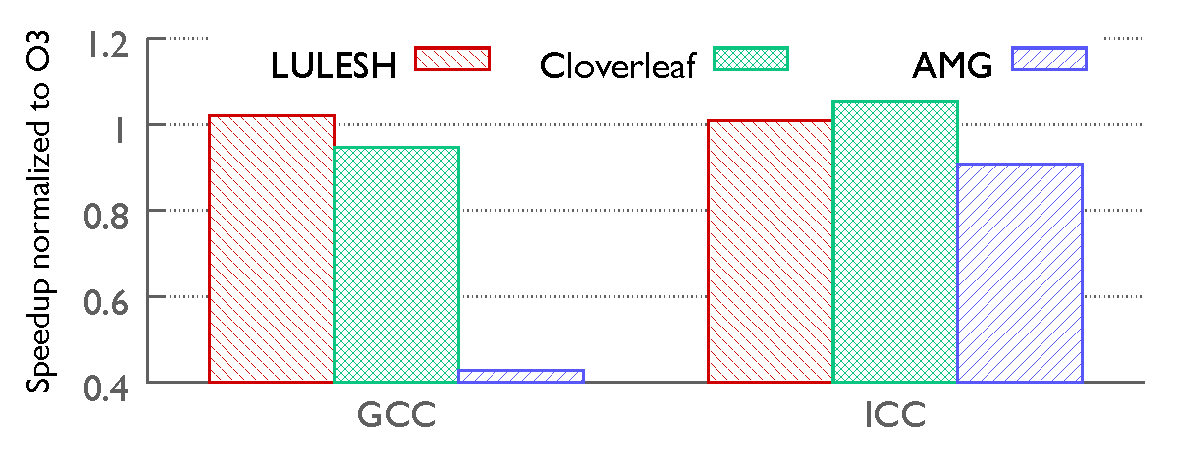
\includegraphics[width=0.7\textwidth]{gnuplot_temp/intro.pdf}
\caption{Combined Elimination does not improve performance significantly.}
\label{fig:ce}
\end{figure}

%
A closer inspection of the experiments for CE revealed that it can
be limited by the results for local minima.  Further, the time
complexity of CE is $O(n^2)$, where $n$ is the number of O3 flags. The
quadratic complexity limits the use of CE for newer GCC versions such
as 5.4.0, which have more than 200 binary optimization flags and 170
multi-valued parameters.  In this work, we address the challenge of
a large search space by employing a novel search space focusing
technique to guide random search.

%In~\cite{PanE06, Pan:2008:taco}, GCC 3.3.3 was evaluated and it has only 38 binary (on/off) options, but it can be much slower for modern GCC, e.g., release 5.4.0, which has more than 200 binary optimization flags and 170 multi-valued parameters.
%In brief, the-state-of-the-art CE is not only time-consuming but also often cannot guarantee performance improvements, as shown in \Cref{fig:ce}.
%coarse-grained random algorithm and fine-grained greedy
%
Fine-grained per-region compilation techniques~\cite{Pan:2008:taco,
  cere, chill, poet} divide a program into different compilation modules and
optimize each separately. 
%
Specifically, source-code level auto-tuners~\cite{chill, poet} focus
on a single simple computation kernel without considering module
interactions in real-world applications. As prior work in compiler flag
selection~\cite{Pan:2008:taco, cere} also assumes that compilation
modules are independent, they assemble an optimized executable by
greedily picking the best code variant of each module. However, the
modules of a program may not be independent due to cross-module
interference, such as shared data structures and link-time
inter-procedural optimizations~\cite{lto, lto2} across multiple
modules.  In particular, link-time optimizations can drive
optimization decisions, such as \emph{loop unrolling}, and may
invalidate earlier transformations that were made independently for
the compilation modules.

{\bf Contributions:}
%
Based on the observations above, we develop a fine-grained auto-tuning
framework, \toolname, that targets modern scientific applications.
%added by Frank
Our overall objective is to extract the best performance out of an
application that is executed repeatedly, such as in high-performance
computing (HPC) where scientists test their hypotheses in experiments
repeatedly with similar inputs using the same algorithms. 
%
To clarify, we {\em neither} attempt to derive a better set of
optimizations for O3, nor do we attempt to generalize a specific set
of optimizations across region boundaries or select different
algorithmic code variants according to input characteristics (in
contract to ~\cite{jiajia,yeom}). Instead, our objective is to 1)
assess whether or not there are module interactions and, if so, 2)
understand how to capitalize on such interactions.

Our target HPC applications exploit multi-core parallelism via OpenMP~\cite{OpenMP}.
Their hot-spots consist of OpenMP loops that account for a significant
fraction of execution time. \toolname outlines these loops and
converts them into individual functions, whose compilation can be
auto-tuned.  To this end, \toolname employs a novel and effective
search space focusing technique to guide random search based
compilation auto-tuning.

%\todo{abstract talks about profiling but not this technique; i think we should say both things in both places.} {changed. Not sure whether it's better.}
%todo{Also, we should mention the search space work earlier when discussing other techniques}{You mean per-region compilation? the advantage is that we want to use it as a direct motivator. If we move it earlier, the transition would be a problem.}
%Our evaluations show that \toolname achieves up to 18.1\% higher
%performance using region-specific optimizations than global O3 flags
%on a set of scientific benchmarks run on several generations of HPC
%architectures.
The contributions of this paper are:
\begin{itemize}
%[leftmargin=6.5mm]
\item We develop a fine-grained per-loop compiler flag selection
  framework, \toolname, that combines program profiling~\cite{caliper}
  % source code transformation, Caliper~\cite{caliper} low-overhead
  % timing infrastructure,
  and search space focusing algorithms to tune hot kernel loops of
  modern scientific programs simultaneously without sacrificing the
  optimization context for production compilers.
  % \todo{too many keywords: also what is source code transformation?
  % i think we can just say light-weight profiling and search space
  % algorithm}
\item We demonstrate that \toolname is able to improve program
  performance for a set of scientific benchmarks by 9.3\% to 10.3\% in
  comparison to the O3 baseline and 4.6\% to 5.6\% relative to prior work,
  both in geometric mean, on several generations of HPC architecture.
%
  %Our \toolname further has the potential to improve machine learning
  %based predictive modeling techniques in the future.
  % \todo{not sure what the potential ML bit is? Can we claim beyond
  % state of the art?} {Previous work show ML never beats random
  % search in terms of program performance improvement}.
\item We conduct an in-depth case study for the Intel compiler tool chain to
  show how fine-grained compiler
  flag selection affects inter-module dependencies and demonstrate
  that it should not be performed greedily, but rather in a focused and targeted manner.
%\todo{is there something specific to Intel? If not, why mention that} {Yes. xiar and xild must be used, and they are not part of ICC}
\end{itemize}

Our \toolname implementation automates these steps, with the
exception of profile instrumentation and collection of timing results,
which are manual in our research prototype, but could be automated
with further engineering effort invested (but are of no research value).

% Paper organization
\iffalse
\todo{I dont think this is useful}
Section \ref{design} first defines terminologies and notations used in this paper, after which \toolname framework and work flow design considerations are explained.
Section \ref{experiment design} gives a brief overview of all experimental settings, such as benchmarks, platforms, and measurement methodology.
The overall tuning results for our benchmark suite are presented in section \ref{results and analysis} to show the effectiveness of \toolname.
Related work is discussed in section \ref{related work}.
Section \ref{conclusion} summarizes this paper and discusses work in detail future work.

iterative compilation~\cite{iterativecompilation, 1191546, 1611551} to search  space of . and auto-tuners~\cite{activeHarmony, opentuner, Zhang:2012:AAS:2259016.2259037}, to take

Motivating example: vectorization or not, to show per-loop compilation may be useful. Can also extract motivation from Peak~\cite{Pan:2008:taco}.

Contribution:

Research questions:
\begin{enumerate}
\item granularity: how to split code
\item stability/sensitivity: R, FR, CFR
\item Effectiveness
\end{enumerate}

Use LULESH as an example for in-depth analysis
\begin{enumerate}
\item why CFR is better than G.realized
\item why CFR is not as good as G.expected
\item Is G.expected a tight upper bound?
\end{enumerate}

Experimental evaluation:
\begin{enumerate}
\item LULESH
\item Cloverleaf
\item AMG
\end{enumerate}

Discussion:

Iterative compilation is a very important compiler-based auto-tuning technology to improve program performance. Search space is too large for exhaustive enumeration. The critical limitation of the state-of-the-art is lack of knowledge of interactions among different compilation flags. It is challenging to automatically derive compiler flag interactions.

Runtime parameter auto-tuning is another effective techniques to improve program performance. Application self-tuning, library auto-tuning, compiler-based code variant tuning. Previous work does not combine iterative compilation and runtime parameter tuning together.

Two possible contributions:
\begin{enumerate}
\item automatically extract compiler flag interactions to reduce space search overhead.
\item combine compile-time and runtime tuning.
\end{enumerate}
\fi


\section{Design of \toolname} \label{design}

This section first defines terminology and notations used throughout this
work and then details the design of the \toolname framework and its
work flow.
\vspace{-1.5mm}
\subsection{Compiler Flag Space Construction}

%how to extract interactions automatically
Modern optimizing compilers feature many internal optimization passes
and expose several hundreds of command-line flags to trigger and
parameterize them.  Each flag can be viewed as a variable with two or
more valid values, i.e., a flag could either be a binary switch
to turn on/off a certain optimization (e.g., loop unrolling and loop
tiling), or a multi-valued parametric option to set pass-specific
parameters (e.g., thresholds for function inlining and algorithmic
variants of register allocation).
%
%compiler flag vector, compiler flag space
The set of all flags composes a space called the compiler optimization
space ($COS$), in which each point is a set of instantiated flags, a
so-called compiler flag vector or compilation vector ($CV$).

Suppose there are $N$ compiler flags, denoted as $F_i$
$(1\leq{i}\leq{N})$.  Further suppose $F_i$ has $n_i$ possible values
$f_{i1}, f_{i2}, ..., f_{i{n_i}}$.  Then a sample $CV$ is represented
as $(F_1=f_{1k_{1}}, F_2=f_{2k_{2}}, ..., F_N=f_{Nk_{N}})$ or simply
$(f_{1k_{1}}, f_{2k_{2}}, ..., f_{Nk_{N}})$, where
$1 \leq{k_i} \leq{n_i}$.  Thus, there are in total
$C_0=\prod_{i=1}^{N} n_{i}$ $CVs$, each of which could be used to
compile all source files of a program in a traditional compilation
model (see \Cref{fig:cm1}).

\begin{figure}
\centering
\subfloat[]
{
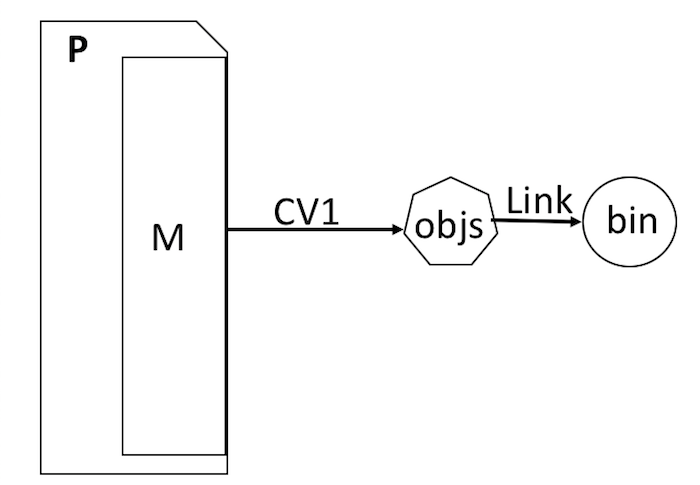
\includegraphics[scale=.2]{figures/cm1.png}
\label{fig:cm1}
}
\subfloat[]
{
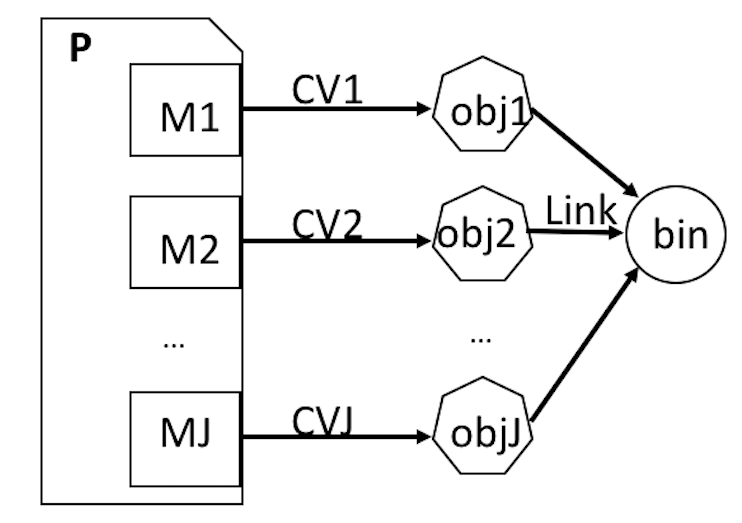
\includegraphics[scale=.2]{figures/cm2.png}
\label{fig:cm2}
}
\caption{Comparison of compilation models. a) A traditional compilation
  model with the same $CV$ to compile all modules; b) \toolname's
  compilation model with different $CVs$ to compile
  different modules.}
\label{fig:cms}
\end{figure}


\if 0
\begin{figure}
\centering
\subfloat[Part 1][]{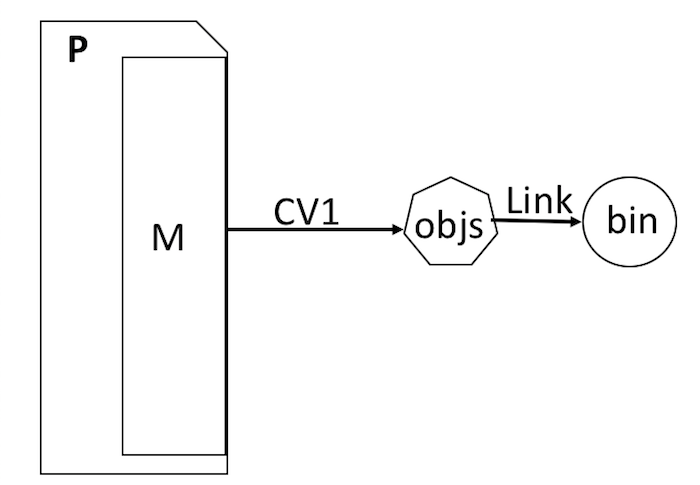
\includegraphics[width=0.4\textwidth]{figures/cm1.png}
\label{fig:cm1}}
\subfloat[Part 1][]{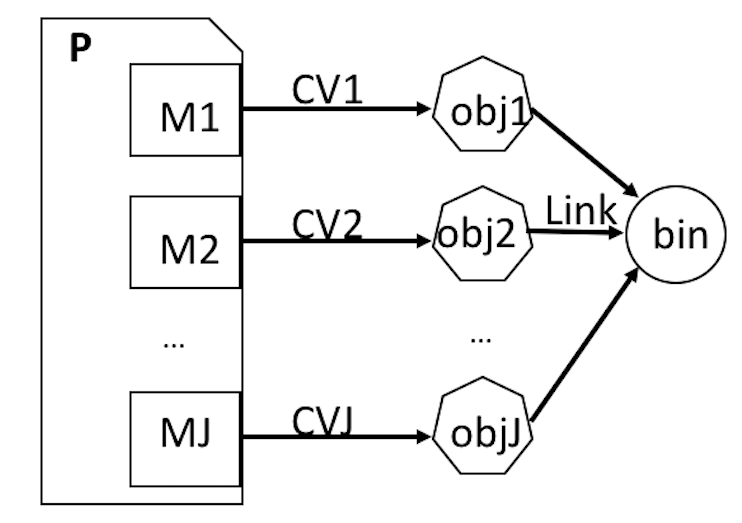
\includegraphics[width=0.4\textwidth]{figures/cm2.png}
\label{fig:cm2}}
\caption{Comparison of compilation models. a) A traditional compilation
  model with the same $CV$ to compile all modules; b) \toolname's
  compilation model with different $CVs$ to compile
  different modules.}
\label{fig:cms}
\vspace{-4mm}
\end{figure}
\fi


\begin {table}[t]
%\nocaptionrule
\caption{Symbol definitions}
\label{table:notations}
%\vspace{2pt}
\centering
\footnotesize
\begin{tabular}{ p{2cm}p{14cm} }
\hline
\textbf{Notation} &  \textbf{Definition} \\ \hline
$N$ & number of compilation flags/options\\ \hline
$F_i$ & i-th compilation options, $(1\leq{i}\leq{N})$\\ 
\hline
$n_i$  & number of possible values for $F_i$ \\ \hline
$f_{ih}$  & h-th value of $F_i$, $(1\leq{h}\leq{n_i})$ \\ 
\hline
$COS$ & Compiler optimization space; Cartesian
   product of values possible for all options:
   ($F_1=f_{11}, F_1=f_{12}, ..., F_1=f_{1n_1})~\times$
    ($F_2=f_{21}, F_1=f_{22}, ..., F_1=f_{2n_2})~\times$
   $\space(...)~\times$ ($F_N=f_{N1}, F_1=f_{N2}, ..., F_1=f_{Nn_N})$\\ \hline
$COS_{new}$& COS for our fine-grained approach\\ \hline
$CV$ & Compilation vector, an instance in $COS$, e.g.,
  $CV=(F_1=f_{11}, F_2=f_{22}, ..., F_N=f_{N3})$\\ \hline
% & \\
 $C_0$ & $\prod_{i=1}^{N} n_{i}$, number of $CV$s in $COS$ \\ \hline
%& \\
$M$ & A \textbf{compilation module} within which source file(s) are compiled with the same $CV$ \\ \hline
%& \\
 $P$  & A source program composed of one or multiple \textbf{compilation module}s\\ \hline
%  & \\
 $J$ & number of modules M in $P$; is a program-specific variable \\ \hline
% & \\
 $C_1$ & ${C_0}^J$, number of $CV$s in $COS_{new}$ \\ \hline
%  & \\
 $M_j$ & j-th compilation module of $P$, $(1\leq{j}\leq{J})$\\
%\hdashline
% $CV_j$ & CV for $M_j$, $(1\leq{j}\leq{J})$\\
%\hdashline
%CVV & vector of all CVs to compilation a program in \\
%& fine-grained compilation model \Cref{fig:cm2}, \\
%  & \\
\hline
 $K$  & number of $CV$ samples \\ \hline
%  & \\
 $P_k$  & $P$ compiled with k-th set of $CVs$  for a \\& given method \\ \hline
%  & \\
 $M_{jk}$  & j-th $M$ of $P_k$.\\ \hline
%  & \\
 $CV_{jk}$  & $CV$ for $M_{jk}$ \\
\hline
%  & \\
 $MCV_k$  & \textbf{program compilation configuration}, configuration of per-module $CV$ for $P_k$;
  If $P_k$ is composed of $(M_{1k}, M_{2k}, ..., M_{Jk}),$
  and its $MCV_k$ is $(CV_{1k}, CV_{2k}, ... ,CV_{Jk}),$ it
  means that every source file within $M_{1k}$ is
  compiled with $CV_{1k}$ and so on\\
\hline
%  & \\
$T_{jk}$  & total accumulated runtime for $M_{jk}$ \\
 \hline
%  & \\
$T_k$  & end-to-end runtime for $P_k$ and $T_k=\sum\limits_{j=1}^{J} T_{jk}$\\
\hline
%  & \\
$T_{O3}$  & end-to-end runtime for $P$ compiled with O3 \\
 \hline
\end{tabular}
\end {table}

Given a program $P$, a traditional compilation model (shown in
\Cref{fig:cm1}) treats all its source files as a single
compilation module $M$, within which the source files are
compiled with the same $CV$.
% Conceptual diagram:
In contrast, as shown in \Cref{fig:cm2}, \toolname divides program $P$
into $J$ compilation modules $M_1, M_2, ..., M_J$; these modules are
created based on the time spent in various regions, in particular
loops, of the program P.  \toolname then compiles $M_j$ with a $CV$,
which is determined independently from other modules and links all
object files to produce the executable.  Our hypothesis is that
different compilation modules may need different $CV$s to obtain the
best performance due to their diverse code structures.
%and the fact that compiler built-in cost models or heuristics do not always make the best decisions.

However, the primary challenge is that the new search space size
$COS_{new}$ increases significantly from $C_0$ to $C_1={C_0}^J$, since
each module can be compiled independently with a different $CV$ in
$COS$.  Exhaustive search is not a viable option within such an
excessively large space while predictive modeling based on machine
learning requires a significant amount of training data and meaningful
features to begin with~\cite{FursinMGL15}. To address this challenge, we design and implement
several algorithms within our framework, as detailed in the rest of this
section.  To facilitate the discussion, we define the notations
in \Cref{table:notations}. We do not differentiate between a program source code
    module and its corresponding object/binary module. Therefore,
    $P_k$ ($M_{jk}$) may represent the source code module or compiled
    program object/binary module, depending on the context.

\subsection{Space Search Algorithms}

\subsubsection{Coarse-grained Random Search}

Coarse-grained Random Search (denoted as Random) does not modify program
source code. As shown in
\Cref{fig:csr}, It utilizes random search within the traditional
compilation model (\Cref{fig:cm1}), i.e., it applies a single $CV$ to
all source files for any program $P$.  In step \textcircled{1}, 1000
$CV$ samples are randomly selected from $COS$~\cite{opentuner}.  In
step \textcircled{2}, each $CV$ is used to compile $P$ to obtain a
code variant, $P_i$.  Thus, we obtain 1000 code variants in total.  In
step \textcircled{3}, runtimes are collected for all code variants.
In the end, the code variant with the least runtime is selected as the final result.
%Coarse-grained random search does not modify $P$'s
%source code, we denote \\it as $R$.
The size of its search space is
$C_0$, as in \Cref{table:notations}.
%, and pseudo code is presented in \textbf{\Cref{alg:csr}}.
\begin{figure}
\centering
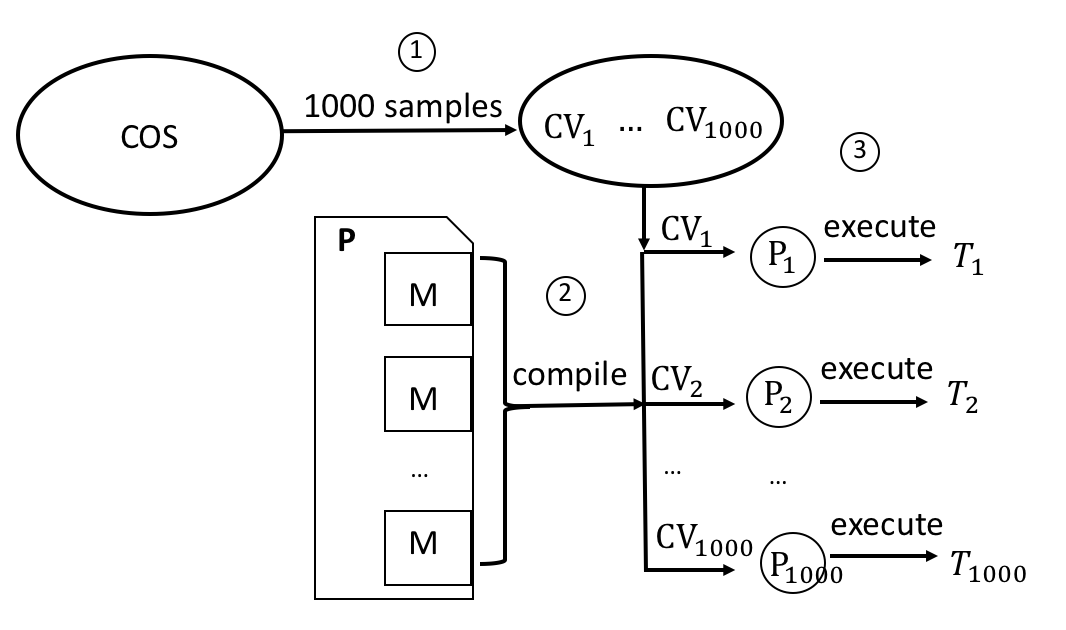
\includegraphics[width=0.6\textwidth]{figures/r_origin}
\vspace{-4mm}
\caption{Overview of Coarse-grained Random Search. $CV_k$ and $P_k$
  with minimal runtime $T_k$ is its final result.}
\label{fig:csr}
\vspace{-4mm}
\end{figure}
\subsubsection{Fine-grained Random Search}

As shown in \Cref{fig:fr}, Fine-grained Random search (denoted as
$FR$) begins with profiling an input program $P$ to identify hot loops
and outlines each of them into a separate source files so that there
are $J$ compilation modules.  After that, $J$ $CV$s are randomly
selected from 1000 pre-sampled $CV$s.  Each selected $CV$ is then used
to compile one of the $J$ modules of $P$.

\iffalse
\begin{algorithm}
\DontPrintSemicolon
\SetAlgoLined
\SetKwInOut{Input}{Input}
\SetKwInOut{Output}{Output}
\Input{$COS, K, P, T_{O3}$}
\Output{$speedup, CV$}
\BlankLine
$k = 0$, $T= [ ]$, $CV$s$ = []$ \;
$CV$s = randomSample ($COS, K$)\;
\While{ $k < K$ }{
    compile $P$ with $CVs[k]$ to generate $P_k$\;
    run $P$ to measure $T_k$ \;
    $T[k] = T_k$ \;
    $k$++
}
$k = \operatorname*{argmin}_k {\{T[k]}$ ${ | 1\leq{k}\leq{K}\}}$ \;
\;
$CV$ = $CVs[k]$\;
speedup = $T_{O3}/T[k]$ \;
\caption{Coarse-grained Random Search}
\label{alg:csr}
\end{algorithm}
\fi

Note that the selection of $J$ CVs and compilation is performed 1000
times in step \textcircled{3} to generated 1000 code variants $P_1$,
..., $P_{1000}$, which are executed to collect runtimes $T_1$, ...,
$T_{1000}$.  In the end, $FR$ reports the code variant with the
minimum runtime as the best version.  
The detailed algorithm is
presented in \Cref{alg:fr}.

\begin{figure}
\centering
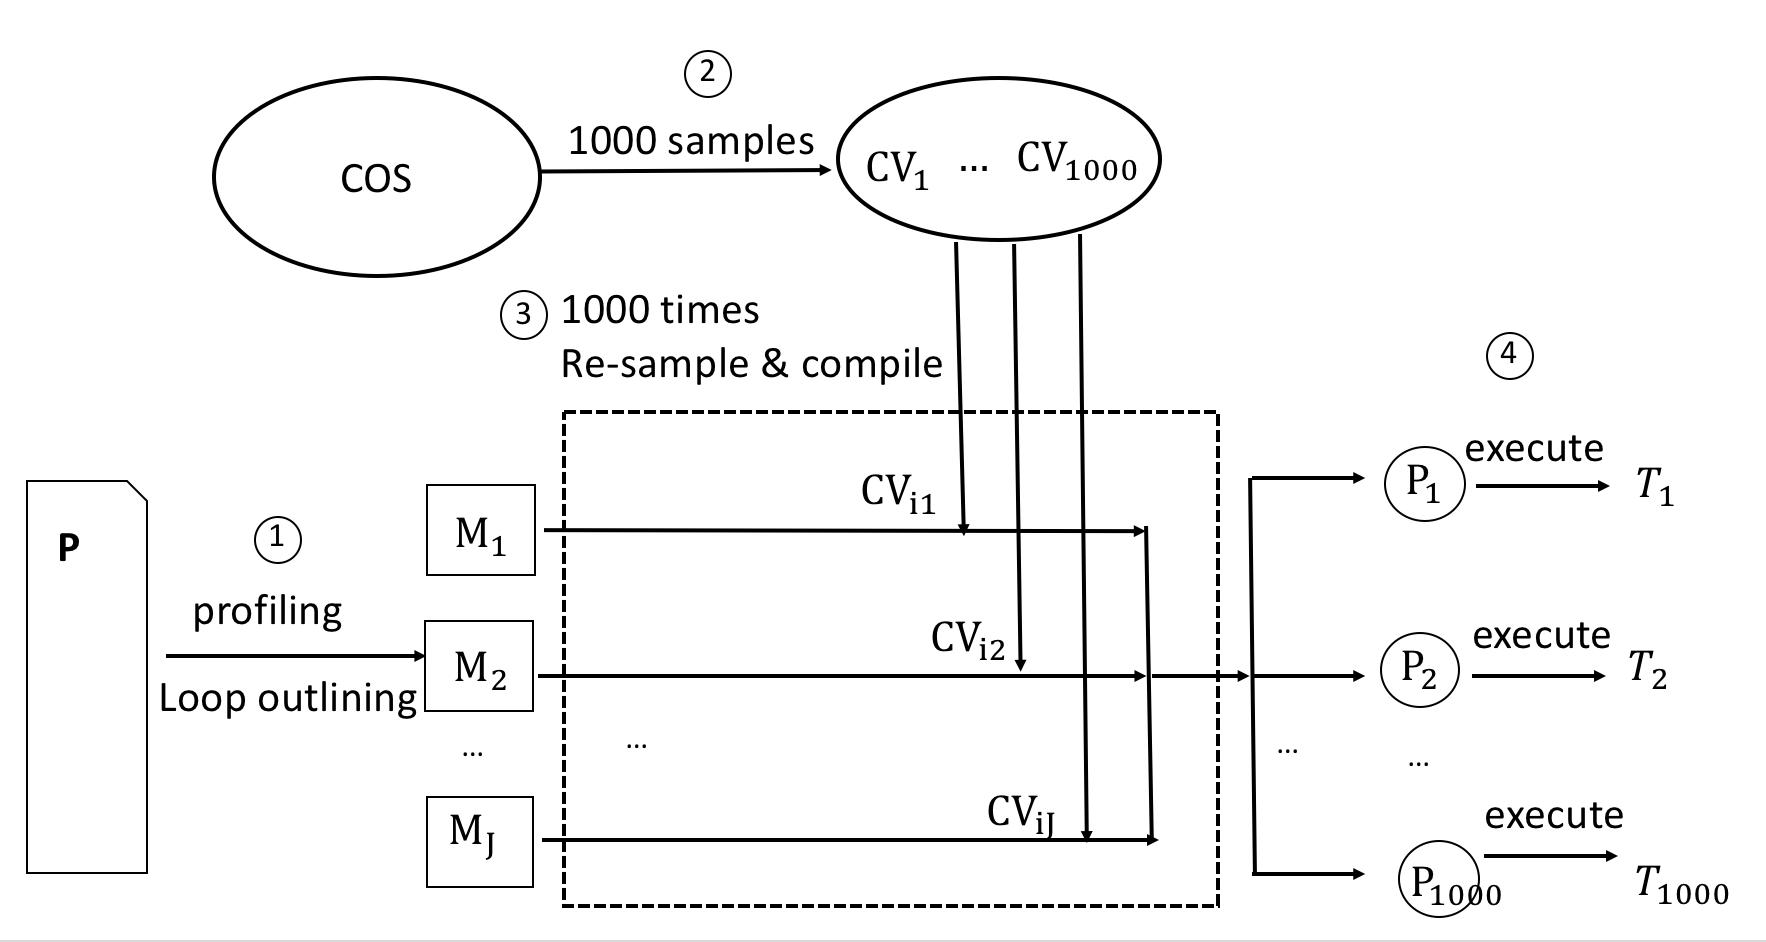
\includegraphics[width=0.6\textwidth]{figures/fr}
\caption{Fine-grained Random Search. Step \textcircled{3} (re-sample \& compile) is performed 1000 times.}
\label{fig:fr}
\end{figure}

\begin{algorithm}
\DontPrintSemicolon
\SetAlgoLined
\SetKwInOut{Input}{Input}
\SetKwInOut{Output}{Output}
//For FR, $CV_{pruned}$ initially is empty\;
\Input{$COS, K, P, T_{O3}$}
\Output{$speedup, CV$}
\BlankLine
$T= [ ]$, $tempCVs=[][]$, $CV$s$ = []$ \;
%\uIf{$CV_{pruned}$ is []}{
//returns K random samples from $COS$\;
$CV$s = randomSample ($COS, K$)\;
%}\Else{
%$CVs = CV_{pruned}$\;
%CFR=true
%}
\For {$k=0$; $k < K$; $k$++}{
    tempCVs[k][] = randomSample($CV$s, $J$)\;
    \For {$j=0$; $j < J$; $j$++}{
    	compile $M_j$ with tempCVs[k][j]
    }
    link $M_1$, ..., $M_J$ to generate $P_k$\;
    run $P_k$ to measure $T_k$ \;
    $T[k] = T_k$ \;
}
$k = \operatorname*{argmin}_k {\{T[k]}$ ${ | 1\leq{k}\leq{K}\}}$ \;
$CV$ = $tempCVs[k]$\;
speedup = $T_{O3}/T[k]$ \;
\caption{Fine-grained Random Search (FR)}
\label{alg:fr}

\end{algorithm}

\subsubsection{Greedy Combination}
% Intuition of Greedy combination

$FR$ does not use the per-loop (i.e. per-module) runtime information.
However, when per-loop runtime information is available, one can
choose better $CV$s for each compilation module.  To this end, we
introduce \toolname, our per-loop runtime collection framework, shown
in \Cref{fig:framework}.  Similar to $FR$, an input program $P$ is first
divided into $J$ compilation modules.  In step \textcircled{2},
\toolname instruments modules via a light-weight~\cite{caliper} API to
measure per-loop runtime.  Then, in step \textcircled{4}, pre-sampled
$CV_1$, ..., $CV_{1000}$ are used to compile $P$ such that all modules
within $P$ are compiled with the same k-th $CV$ to generate $P_k$.  In
step \textcircled{5}, the generated 1000 code variants are then
executed to collect per-loop runtimes, which are represented as
$T_{jk}$ for accumulative runtimes per compilation module $M_j$ of
code variant $P_k$.

The intuition of Greedy Combination (denoted as $G$) is to assemble
the final executable by picking the fastest code variant for each module
and linking them together, assuming that their composition produces
the fastest executable with the shortest end-to-end runtime.  Formally,
$G$ chooses the i-th $CV$ to compile $M_j$ such that
$i = \operatorname*{argmin}_k {\{T_{jk} | 1\leq{k}\leq{1000}\}}$, and
then links all object modules to produce the target executable.  The
pseudo code for both the \toolname data collection framework and
Greedy Combination is presented in \Cref{alg:greedy}.

\begin{figure}
\centering
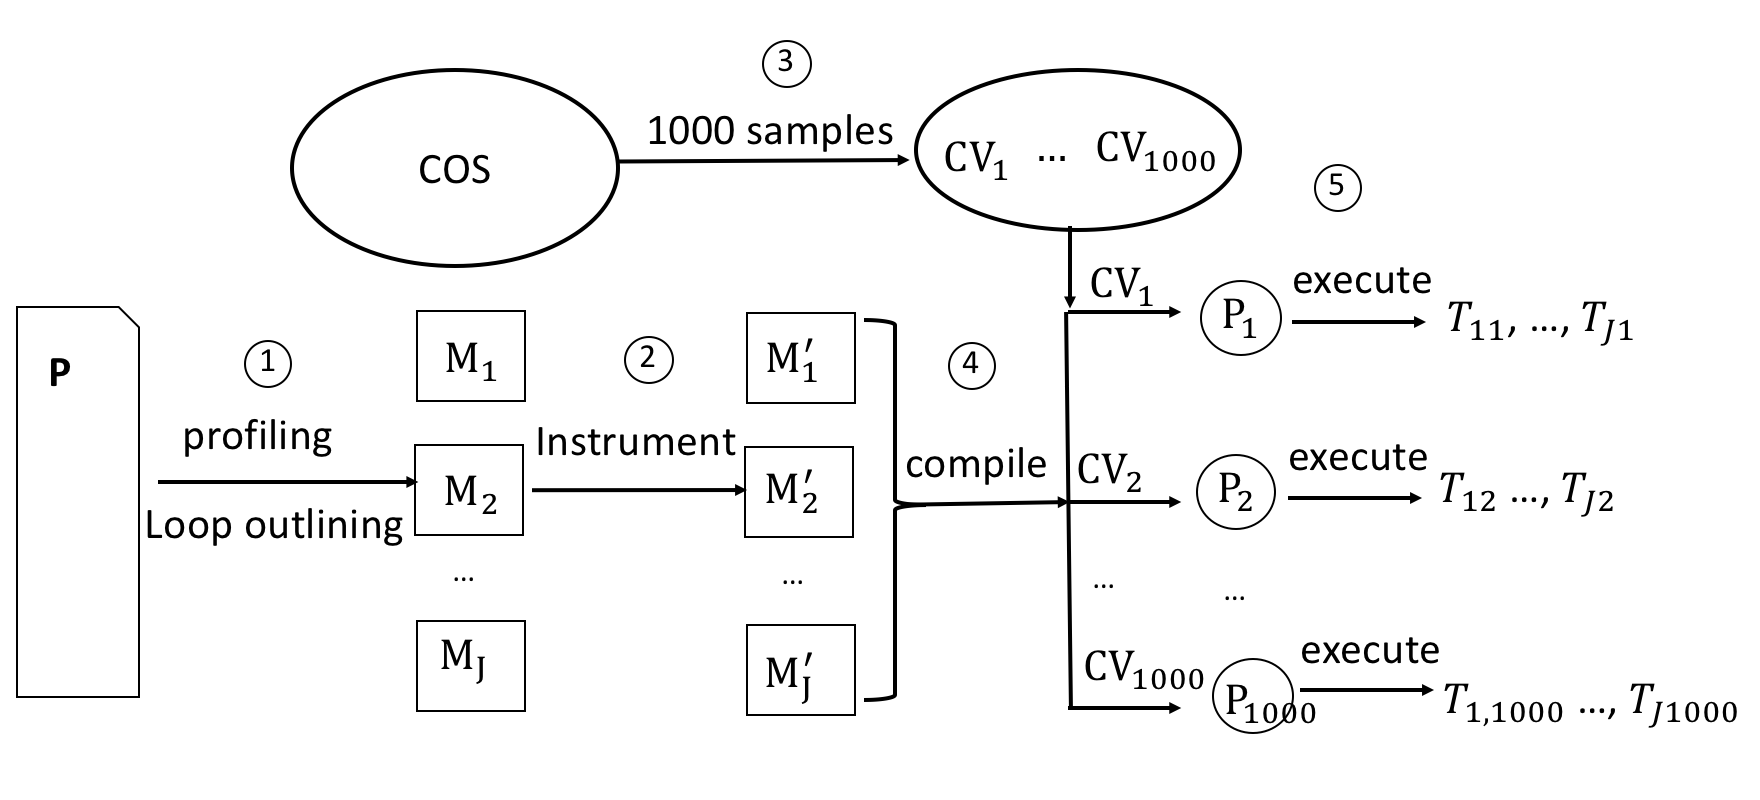
\includegraphics[width=0.6\textwidth]{figures/framework}
\caption{FuncyTuner Per-loop Runtime Data Collection Framework used for
  both Greedy Combination (\Cref{alg:greedy}) and CFR (\Cref{alg:cfr}).}
\label{fig:framework}
\end{figure}

\begin{algorithm}
\DontPrintSemicolon
\SetAlgoLined
\SetKwInOut{Input}{Input}
\SetKwInOut{Output}{Output}
\Input{$COS, K, P, T_{O3}$}
\Output{$speedup, CV$}
\BlankLine
$T = [][]$, $CV$s$ = []$, $CV_{greedy} = []$ \;
$CV$s = randomSample ($COS, K$)\;
$//$ \toolname per-loop runtime data collection\;
%\While{ $k < K$ }{
\For {$k=0$; $k < K$; $k$++}{
    compile $P$ with $CVs[k]$ to generate $P_k$\;
    run $P$ to measure $T_{1k}, ..., T_{Jk}$ \;
    \For {$j=0$; $j < J$; $j++$}{
    	$T[j][k] = T_{{j+1}k}$ \;
    }
}
//Greedy combination\;
\For {$j=0$; $j < J$; $j++$}{
	$CV_{greedy}[j] = \operatorname*{argmin}_k {\{T_{jk} | 1\leq{k}\leq{K}\}}$\;
    compile $M_j$ with $CV_{greedy}[j]$ for bject file $O_j$
}
link $O_j$s to generate target program $P_t$\;
execute $P_t$ to obtain $T_t$\;
$CV$ = $CV_{greedy}$\;
speedup = $T_{O3}/T_t$ \;
\caption{Greedy Combination (G)}
\label{alg:greedy}
\end{algorithm}

\subsubsection{Caliper-guided Random Search}

% \todo{this is unclear; algorithm seems incomplete with an if (true);
% also, i dont think algorithm 1 preserves module to module matching
% of flags}{Nice Catch!}
Similar to $G$, Caliper-guided Random Search (denoted as $CFR$)
depends on \toolname's per-loop runtime data collection to make
informed selection of $CV$s (see \Cref{fig:framework}).  However, the
key difference is that $CFR$ examines more code variants than $G$,
which only greedily assembles and evaluates 1 code variant.  Compared
to $FR$, which does not use any per-loop information and uniformly
performs a random search within the pre-sampled 1000 $CVs$ for each
hot loop, $CFR$ takes advantage of per-loop timing information and
prunes the pre-sampled search space for each hot loop before
re-sampling per-loop $CV$s (line 8 of \Cref{alg:cfr}).  The
intuition is that more performant $CV$s, which generate faster
per-loop code variants, should be kept in the re-sampled search space,
because they may have a higher chance to compose a performant target
executable.  Within this algorithmic framework, $G$ can be
considered as only selecting the top-1 $CV$s, and that $FR$ selects
all 1000 or the top-1000 $CV$s, while $CFR$ selects the top-X
($1<X<<1000$) $CV$s, all on a per-loop basis.  The pseudo code of CFR
is presented in \Cref{alg:cfr}, which also uses the \toolname per-loop
runtime data collection of \Cref{alg:greedy}.

To summarize, Random and G are the state-of-the-art search-based
algorithms while we propose FR and CFR.

\begin{algorithm}[t]
\DontPrintSemicolon
\SetAlgoLined
\SetKwInOut{Input}{Input}
\SetKwInOut{Output}{Output}
\Input{$COS, K, P, X, T_{O3}$}
\Output{$speedup, CV$}
\BlankLine
$k = 1$, $T= [ ]$, $CV$s$ = []$ , $CV_{pruned} = [][]$\;
$CV$s = randomSample ($COS, K$)\;
//step-1: \toolname per-loop data collection (Alg.\ref{alg:greedy})\;
\vspace{.5em}
//prune pre-sampled 1000 CVs\;
\For {$j=0$; $j < J$; $j$++}{
$CV_{pruned}[j][] = $ $\{{CVs[i]\,\,|\,\,T[j][i]}\,\, is\,\,among\,top\, X$-$\,smallest\,\,in\,\,T[j][0]\,,...,\,T[j][K-1]\}$
}
%\If{true}{done}
\For {$k=0$; $k < K$; $k$++}{
	//re-sampling per-loop cv in pruned space.\;
	\For {$j=0$; $j < J$; $j$++}{
    	tempCVs[k][j] = randomSample($CV_{pruned}[j]$, 1)\;
    }
    \For {$j=0$; $j < J$; $j$++}{
    	compile $M_j$ with tempCVs[k][j]
    }
    link $M_1$, ..., $M_J$ to generate $P_k$\;
    run $P_k$ to measure $T_k$ \;
    $T[k] = T_k$ \;
}
$k = \operatorname*{argmin}_k {\{T[k]}$ ${ | 1\leq{k}\leq{K}\}}$ \;
$CV$ = $tempCVs[k]$\;
speedup = $T_{O3}/T[k]$ \;
%Invoke \textbf{\Cref{alg:fr}} with (COS=[], K, P, $T_{O3}$, $CV_{pruned}$)
\caption{Caliper-guided Random Search (CFR)}
\label{alg:cfr}

\end{algorithm}

\section{Experimental Design} \label{experiment design}

In order to evaluate the efficacy of schemes presented in
Section~\ref{design}, we have performed experiments for seven benchmarks
on three architectures. This section describes the
setup used in our experiments.

\subsection{Systems and Benchmarks}

We conducted our experiments on three platforms: AMD Opteron, Intel Sandy Bridge,
and Intel Broadwell.  The architectural
details for these systems are provided in \Cref{settings}.
Our benchmark suite (see \Cref{table:apps}) consists of seven
HPC programs: AMG~\cite{amg2013}, LULESH
\cite{LULESH}, Cloverleaf (CL)~\cite{cloverleaf}, 351.bwaves, 362.fma3d,
363.swim~\cite{specomp2012} and Optewe~\cite{sc2017}.  Three of these benchmarks (bwaves, fma3d, and
swim) are from the SPEC OMP 2012 suite, while the rest are widely used HPC
proxy applications.  These benchmarks have been
selected based on two criteria.  First, they are written in different
languages and exploit multi-core parallelism suitable for HPC via
OpenMP pragmas.  Second, they feature more than one hot loop, which
resembles realistic applications (unlike many other benchmarks with
just a single hot loop). While multiple hot loops present difficulties
for the compiler in coordinating various loop optimizations,
they also provide opportunity to optimize different parts of the code differently.
%
%dvfs, dct
%Benchmark description
%Input selection
% We also report standard deviations in \Cref{table:stdB},
% \Cref{table:stdS} and \Cref{table:stdO}.

All our experiments have been run on CentOS Linux 7.3.1611 and the benchmarks
were compiled
with the Intel C/C++ Compiler 17.04. OpenMP thread placement has been set to
``fine, proclist=[...] explicit'', where proclist is specified in \Cref{settings}.
%
Details of the OpenMP configurations are presented in \Cref{settings}.
Scientific codes follow a time-step execution pattern repeatedly
performing approximations with decreasing numerical error in an outer
loop. Hence, we only run for a small number of time-steps (seconds)
and then exit prematurely once we have obtained a stable execution
time for a time-step. Any optimization then scales up to a full run
over all time-steps (hours). To this end, input sizes and time-steps
(iteration counts of simulation outer loop) have been adjusted so that
every single run is less than 30 seconds for O3 baseline
compilation. In the first experiments (\Cref{cv sensitivity}, ~\Cref{overallResults} and ~\Cref{beatPGO}), we use the same inputs for
tuning and testing; in later experiments, we evaluate the impact of
different inputs (\Cref{inputsensitivity}).

\begin{comment}
Note that 
To account for run-to-run variability, each code variant is executed
10 times and their average is presented as the representative runtime.
\end{comment}

\begin {table}[t]
%\nocaptionrule
\caption{List of benchmarks. LOC: lines of source code.}
\vspace{-2mm}
\centering
{\footnotesize
\label{table:apps}
\begin{tabular}{ p{2.5cm}p{2cm}p{1cm}p{7.1cm}}
%\hline
%  & \\
\textbf{Name} & \textbf{Language} & \textbf{LOC} &  \textbf{ Domain} \\
\hline
AMG & C & 113k & Math: linear solver \\ \hline
LULESH & C++ & 7.2k & Hydrodynamics \\ \hline
Cloverleaf (CL) & C, Fortran & 14.5k & Hydrodynamics\\ \hline
351.bwaves & Fortran& 1.2k & Computational fluid dynamics, SPEC OMP 2012 \\ \hline
362.fma3d & Fortran& 62k & Mechanical response simulation, SPEC OMP 2012 \\ \hline
363.swim & Fortran& 0.5k & Weather prediction, SPEC OMP 2012 \\ \hline
Optewe & C++& 2.7k & Seismic wave simulation \\ \hline
\end{tabular}
}
\end {table}


% why LULESH on Opteron does not bring any performance benefit?
\begin{comment}

\begin{figure*}
%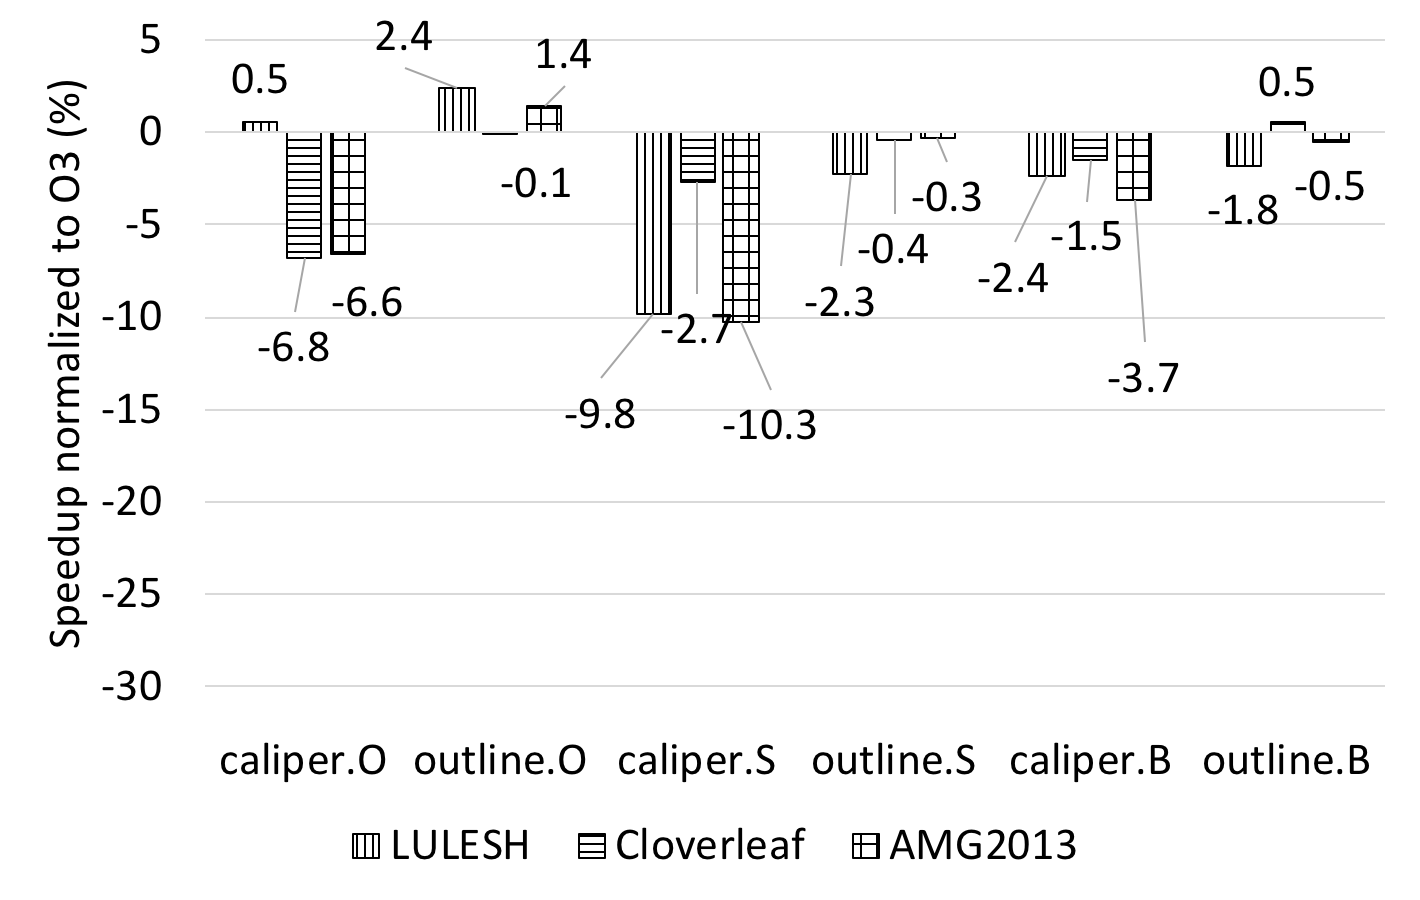
\includegraphics[width=\linewidth]{figures/overhead_all}
%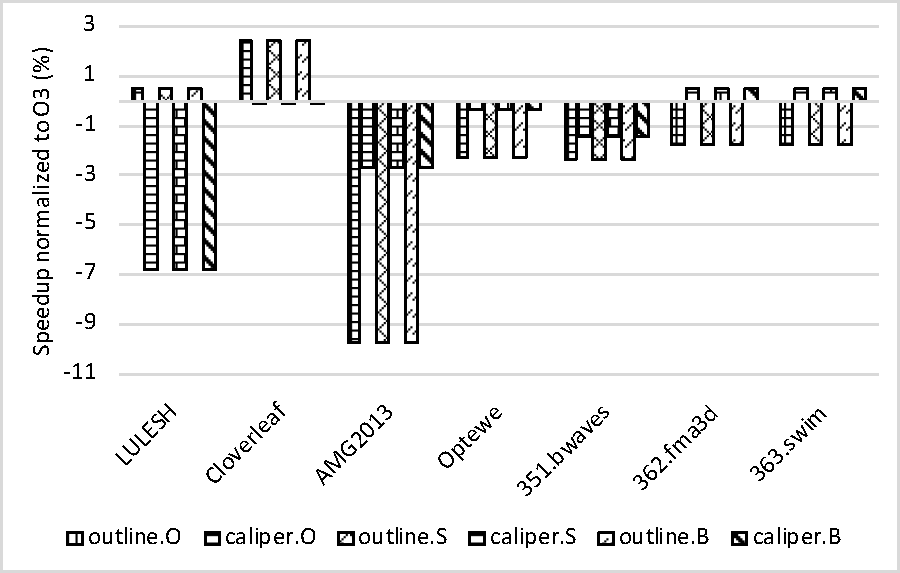
\includegraphics[width=\linewidth]{figures/overhead}
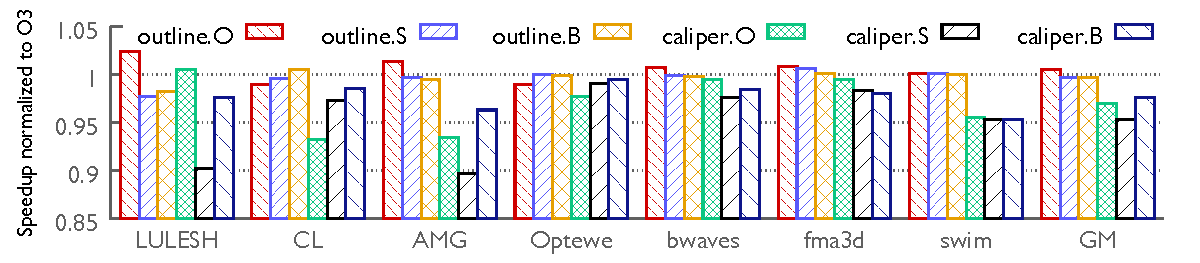
\includegraphics[width=\linewidth]
{gnuplot_temp/overheads.pdf}
\caption{Overheads of loop outlining and Caliper instrumentation on Opteron
  (O), Sandy Bridge (S), and Broadwell (B): outlining results in minimal
  overheads (up to 3\%), but instrumentation can cause noticeable impact.}
\label{fig:overhead}
\end{figure*}

\end{comment}

\subsection{Compiler Flag Selection}

We experiment with 33 optimization-related compilation
flags of the Intel compiler~\cite{icc17manual}.  For flags that
support any value in a continuous range as input, we discretize the
values in the given range.  Then, for each flag $F_i$, \toolname
selects a value $f_i$ from $f_{i1}, f_{i2}, ..., f_{i{n_i}}$ with
equal probability.  A $CV$ is constructed by concatenating the
selected values for all $F_i$s~\cite{opentuner}.  We had to consider
several restrictions when selecting the flags.  First, a flag must not
prevent a program from running successfully on a given target
architecture.  For example, use of the {\em fpack} flag generates code
variants that cause a segmentation fault at runtime and thus {\em fpack } is
excluded.  Second, for fair performance comparison among different
code variants, \toolname enforces strict floating point
reproducibility by discarding floating point related optimization
flags, and always uses {\em -fp-model source } in the presented results.  Last,
optimized library options, such as Intel MKL and IPP
related linkage options, are also excluded since they are not used by
our benchmarks.

Also, in order to reach the full optimization potential of the Intel
compiler tool chain, according to the Intel optimization
note~\cite{iccOpt}, Intel's linker xild and library archive tool xiar
should be used.  We thus modify build systems of all benchmarks
accordingly.
%to meet these practical standards.
Processor-specific flags are also considered for best performance on
each architecture.

\begin{comment}
\begin {table}
%\nocaptionrule
\caption{Notations for code variants. \emph{original}: the unmodified source code; \emph{outlined}: code with hot loops outlined; \emph{caliper}: code with Caliper instrumentation calls; \emph{O3}: the code is compiled with O3 baseline CV.} \label{table:algs}
%\vspace{2pt}
\centering
\begin{tabular}{ l|l }
%\hline
%  & \\
\textbf{Notation} &  \textbf{Definition} \\
\hline
$O3$ &O3, original\\
\hline
$O3.outlined$ &O3, outlined\\
\hline
$O3.caliper$ &O3, outlined and instrumented\\
\hline
$R$ & R, original\\
\hline
\multirow{3}{*}{$G.expected$}
 & Expected runtime of Greedy algorithm.\\
 & $T_{G.expected}=\sum\limits_{j=1}^{J} T_{j{k_j}}$, and\\
 & $k_j=\operatorname*{argmin}_k {\{T_{jk} | 1\leq{k}\leq{K}\}}$\\
\hline
$G.realized$ & Greedy algorithm, outlined\\
\hline
$FR$ &FR, outlined\\
\hline
$Overall$ & CFR, outlined, non-loop code $CV$s with \\
& top-30 lowest end-to-end runtime $T_k$\\
\hline
$Nonloop$ & CFR, outlined, non-loop code $CV$s with \\
& top-30 lowest non-loop code runtime\\
\hline
$Merged$ & CFR, outlined, non-loop code $CV$s \\
&from CFR Overall and Nonloop\\
\hline
$CFR$ & same as CFR merged\\
\hline
\end{tabular}
\end {table}
\end{comment}
% Experimental configurations
\begin{table}[t]
\centering
\caption{Platform overview, runtime configurations, and benchmark inputs.}
%\vspace{-3mm}
%Intel Xeon Phi is configured as Quadrant-Cache mode w/ 16GB MC-DRAM as LLC, which is fastest for our benchmarks.}
\label{settings}
%\bigskip
{
\footnotesize
\begin{tabular}{ p{6.1cm}p{2.2cm}p{2.8cm}p{2.5cm} }
\specialrule{.2em}{.1em}{.1em}
\bf{Machine} &AMD Opteron & Intel Sandy Bridge & Intel Broadwell \\
\hline
\bf{Processor} & Opteron 6128 & Xeon E5-2650 0 & Xeon E5-2620 v4\\
\bf{Sockets} & 2 & 2 & 2 \\
\bf{NUMA nodes} & 4 & 2 & 2  \\
\bf {Cores/Socket} & 4 & 8 & 8  \\
\bf{Threads/Core} & 2 & 2 & 2 \\
\bf{Core Frequency [GHz]} & 2.0 & 2.0 & 2.1  \\
\bf{processor-specific flag} & default & -xAVX & -xCORE-AVX2 \\
\bf{Memory size [GB]} & 32 & 16 & 64\\
\bf{OpenMP thread count} & 16 & 16 & 16\\
\bf{OpenMP thread proclist} & [0-15] & [0-15] & [0-31:2] \\
\bf {LULESH: input size, time-steps} & 120, 10 & 150, 10 & 200, 10 \\
\bf {Cloverleaf: input size, time-steps} & 2000,30 & 2000,30 & 2000,60 \\
\bf {AMG: input size} & 18 & 20 & 25 \\
\bf {Optewe: input size, time-steps} & 320, 5 & 384, 5 & 512, 5 \\
\bf {bwaves: input, time-steps} & train, 10 & train, 15 & train, 50 \\
\bf {fma3d: input} & train & train & train \\
\bf {swim: input} & train & train & train \\
\specialrule{.2em}{.1em}{.1em}
\end{tabular}
}
\vspace{-2mm}
\end{table}

\subsection{Loop Outlining and Caliper Instrumentation}

In order to find code regions that need to be outlined, i.e., separated
into individual modules, \toolname profiles the target application
compiled with ``-O3 -qopenmp -fp-model source''  to identify hot loops.  The profiling is done using
Caliper's instrumentation API~\cite{caliper}, which returns the
per-loop runtime. Only loops whose runtime is at the least 1.0\% of
the baseline's end-to-end runtime, are outlined as independent
compilation modules. Runtime for code other than the hot loops
(non-loop code) cannot be directly measured because such code tend
to be scattered across many source files.  Thus, non-loop code runtime
is derived by subtracting the aggregate runtime of hot loops from
program end-to-end runtime for a given code variant.
%
Caliper instrumentations generally introduce less than 3\% overhead
and the per-loop runtimes are sufficiently informative to \toolname
so that measurement noise is tolerated with its search
algorithms.
%All code variants used in our experiments are listed in
%\Cref{table:algs}.
To evaluate performance, we use ``-O3 -qopenmp -fp-model source'' CV  as
the baseline and report speedup relative to this
baseline unless otherwise specified.  We also note that data points marked {\em
G.expected} are calculated by summing up the best per-loop and non-loop
code runtimes obtained with different compiler options.
%
They are used as an estimation of the upper bound for the Greedy
algorithm. However, this is a hypothetical bound assuming pairwise
independence among different compilation modules. The bound serves as
a reference to assess this independence assumption.


\section{Results and Analysis}

\label{results and analysis}

%Several factors impact the performance under \toolname:
%overhead of outlining and profiling, non-loop code, characteristics of applications, etc.
%In this section, we study these factors and compare the benefits of optimizing
%compilation using traditional coarse-grained random search (R), Fine-grained random search
%(FR), Greedy Combination (G), and Caliper-guided random search (CFR).
\begin{comment}
\subsection{Analysis of Overheads}
The outlining of hot loops into functions by Fine-grained Random Search (FR),
Greedy Combination (G), and Caliper-guided Random Search (CFR)
may affect inter-procedural
optimization (IPO).  Moreover, G and CFR rely on per-loop profiling
information to identify performant CVs.
%
Measurement overhead is inevitable in such scenarios due to
the use of instrumentation.  To
assess these costs, we compare the runtime of code variants subject to
such overhead with the baseline version and report the results in
\Cref{fig:overhead}.  We observe the following trends in these
results:

\vspace{.25em}
\noindent 1) Outlining hot loops typically introduces less than a 3\%
penalty on program performance across all architectures in our
experiments.
%, even though inter-module ipo is enabled by default for O3 baselines.
%The slowdowns on Intel Knights Landing (KNL) for LULESH is -22.5\%.
%We consider such a big slowdown as a performance bug of ICC/ICPC.
%Investigation of the root cause is out of this work's scope, thus we leave it as future work.
In fact, on AMD Opteron, we observe marginal performance improvements
for LULESH and AMG.
% Excluding the exceptional case of LULESH on KNL, we
Based on these results, we conclude that loop outlining can be done at
a low cost, which can often be offset by gains obtained using our
\toolname approach.

\vspace{.25em}
\noindent 2) Caliper instrumentation incurs less than 10\% slowdown
across all benchmarks and architectures.
% , but introduces 29.7\% and 18.1\% penalty to LULESH and Cloverleaf
% on KNL, respectively.  We suspect the slowdown of LULESH is due to
% the aforementioned ICC performance bug.  Slowdown of Cleverleaf can
% be attributed to two factors: the high synchronization overhead of
% KNL due to high number of threads and too many timing samples are
% taken for Cloverleaf (2.6X more than AMG because of more hot loops
% and invocations).
While reasonably low relative to the overall runtime, such a measurement
overhead can induce inaccuracy in the measured runtimes and
impact results of G and CFR.  We further discuss this issue in
\Cref{cv sensitivity,overallResults}.
\end{comment}

\begin{comment}
\begin{figure}
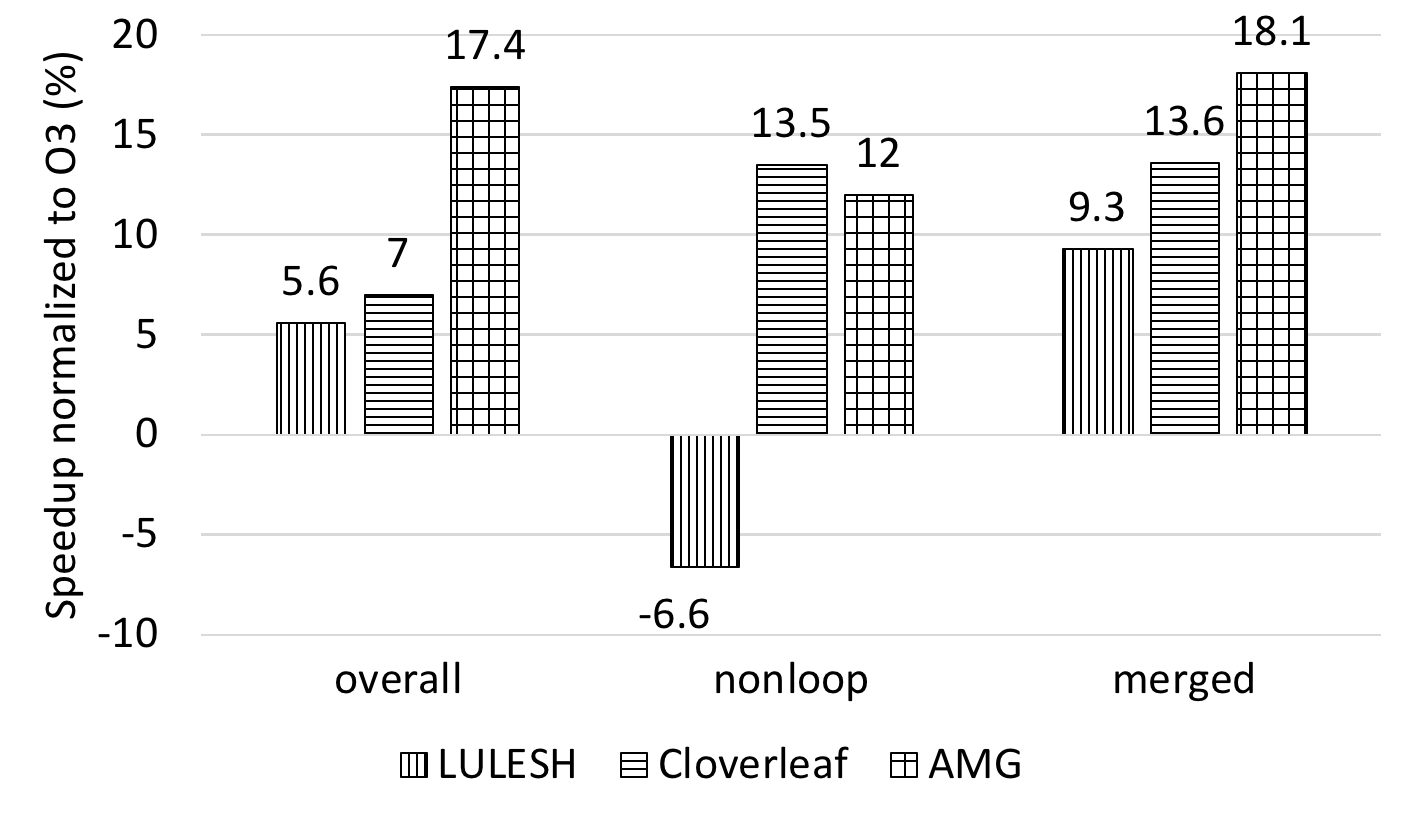
\includegraphics[width=\linewidth]{figures/sensitivity_opteron}
\caption{Benefit of Merged Non-Loop code CVs for CFR on AMD Opteron}
\label{fig:sensitivityOpteron}

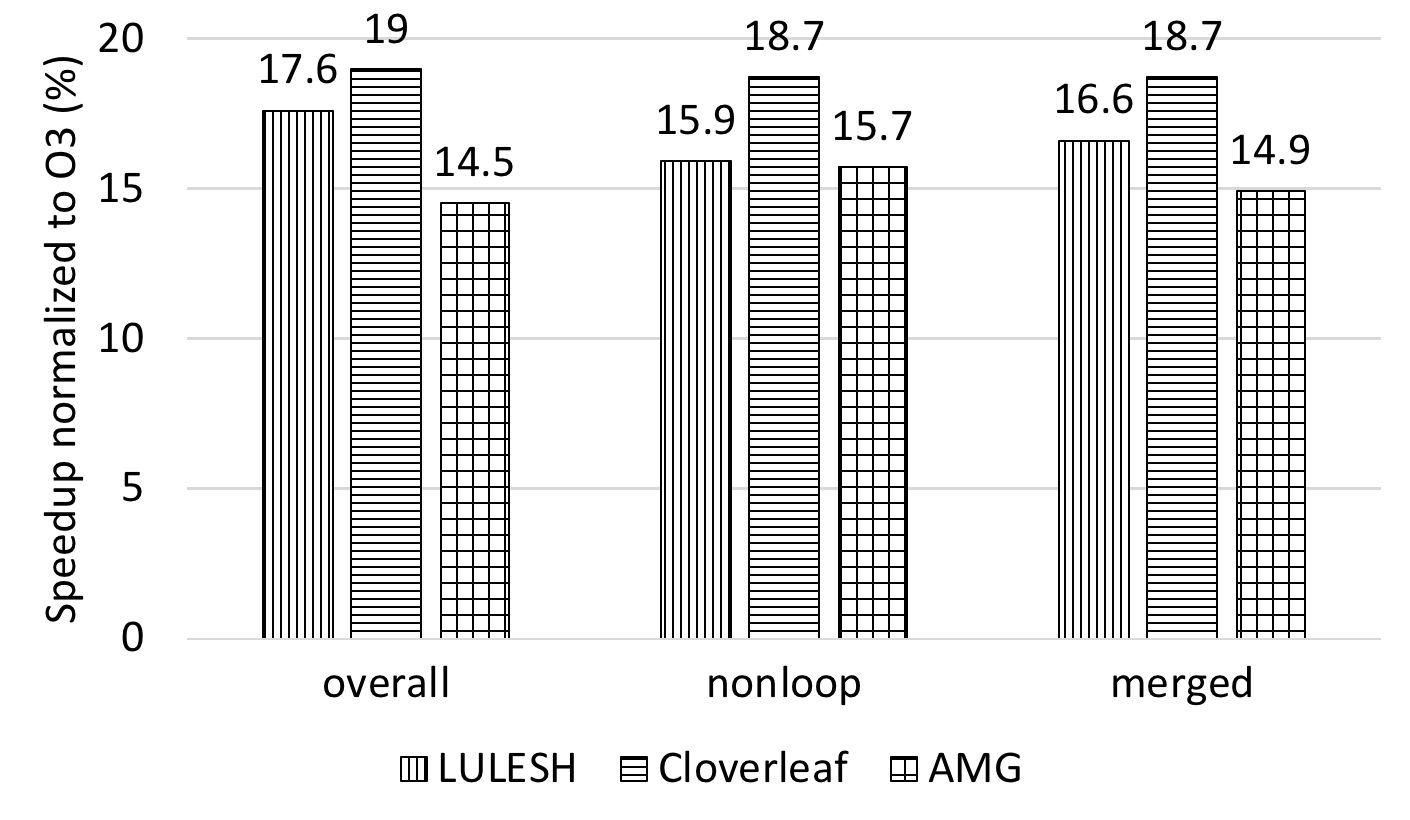
\includegraphics[width=\linewidth]{figures/sensitivity_sandy}
\caption{Benefit of Merged Non-Loop code CVs for CFR on Intel Sandy Bridge}
\label{fig:sensitivitySandy}

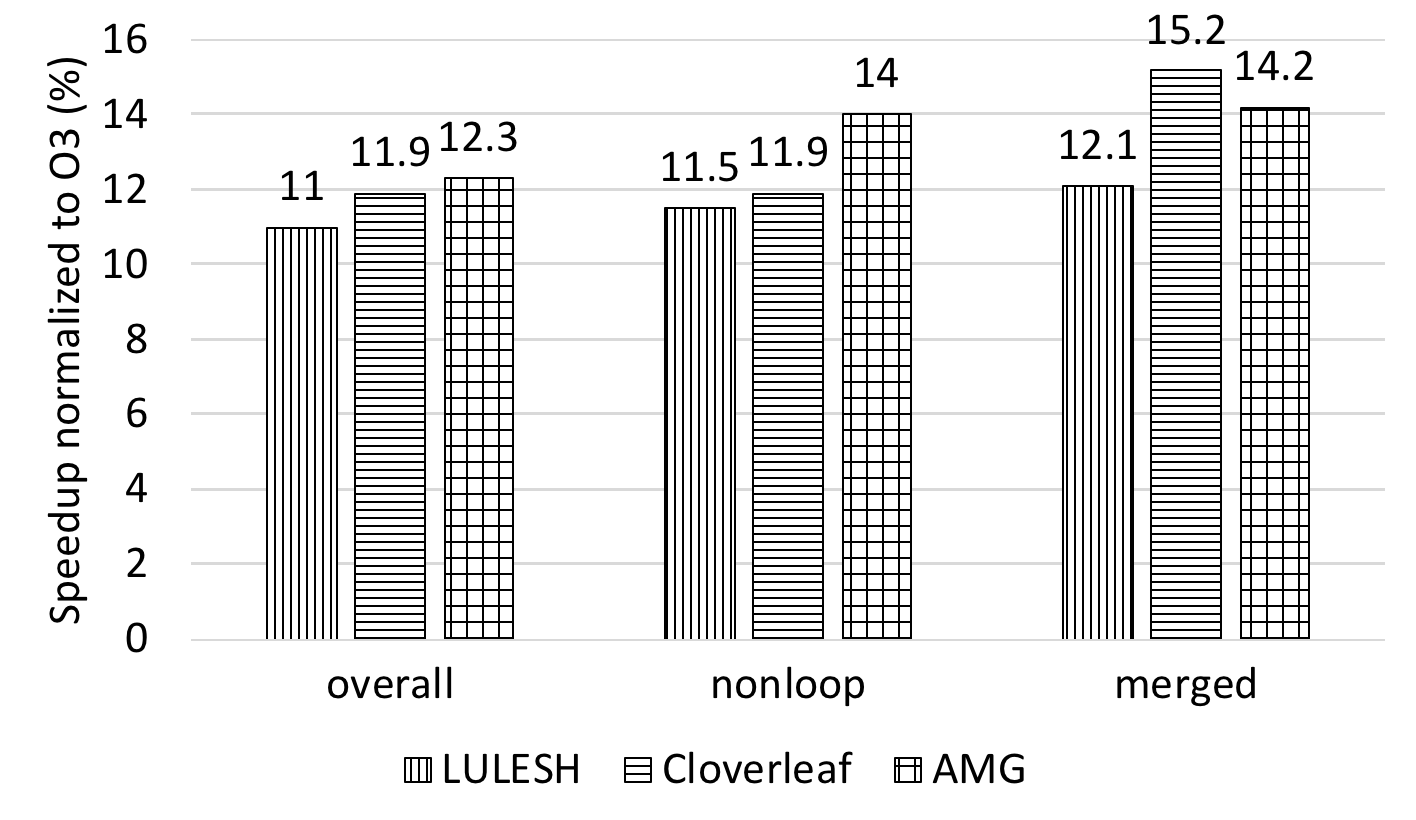
\includegraphics[width=\linewidth]{figures/sensitivity_broadwell}
\caption{Benefit of Merged Non-Loop code CVs for CFR on Intel Broadwell}
\label{fig:sensitivityBroadwell}
\end{figure}
\end{comment}

\subsection{Sensitivity of Non-loop Code CVs}\label{cv sensitivity}

%Motivation
%As discussed, measurement error is calling for tolerance from
%\toolname search algorithms.
In our initial experiments, we found that even when the runtime spent in the
non-loop codes is a small fraction of the total runtime,
the choice of CVs for them can be vital to the overall performance
improvement.
Further, since we derive the non-loop runtime by subtracting the
runtimes of hot loops from the program end-to-end runtime, it also
includes the Caliper instrumentation overhead.  If this overhead is
much higher than the actual non-loop runtime, the derived non-loop
runtime may not be a good indicator for selecting the non-loop CVs
aimed at optimizing production runs that do not include Caliper
instrumentation. This issue may impact the performance improvements due to search
algorithms that rely on such information, i.e., CFR.

An alternative
metric to identify performant CVs for non-loop code is the program
end-to-end runtime since it is a good indicator of how non-loop and
hot-loop CVs interact.
Comparisons for CFR variants in \Cref{fig:sensitivity}
shows that, typically, both derived non-loop time (denoted
as \emph{Non-loop}) and end-to-end runtime (denoted as
\emph{Overall}) result in a significant performance improvement,
when used as the non-loop code runtime metric.  However, we obtain
 performance degradation in one case -- LULESH on Opteron -- if the
derived non-loop time metric is used.  Further, we find that
neither of these two metrics outperforms the other for all cases.
\vspace{2pt}
\begin{figure}
\centering
\subfloat[Comparison on AMD Opteron]{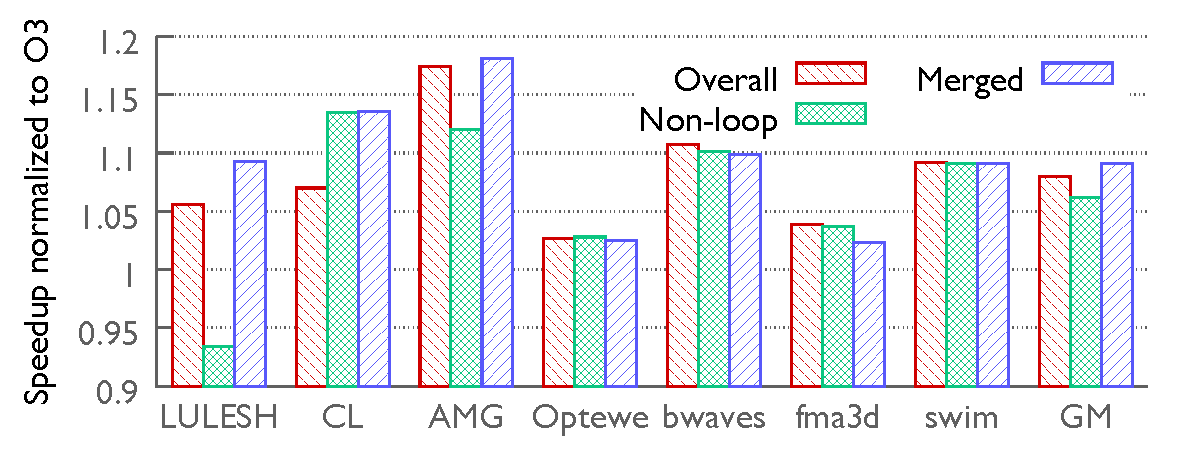
\includegraphics[scale=.4]
{gnuplot_temp/fc_opteron.pdf}
\label{fig:sensitivityOpteron}}
\subfloat[Comparison on Intel Sandy Bridge]{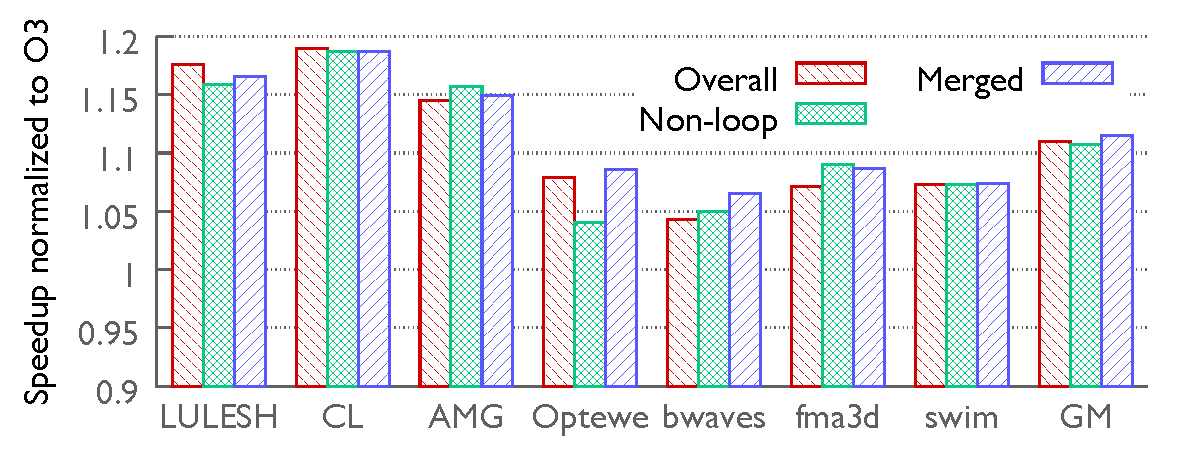
\includegraphics[scale=.4]
{gnuplot_temp/fc_sandy.pdf}
\label{fig:sensitivitySandy}}

\subfloat[Comparison on Intel Broadwell]{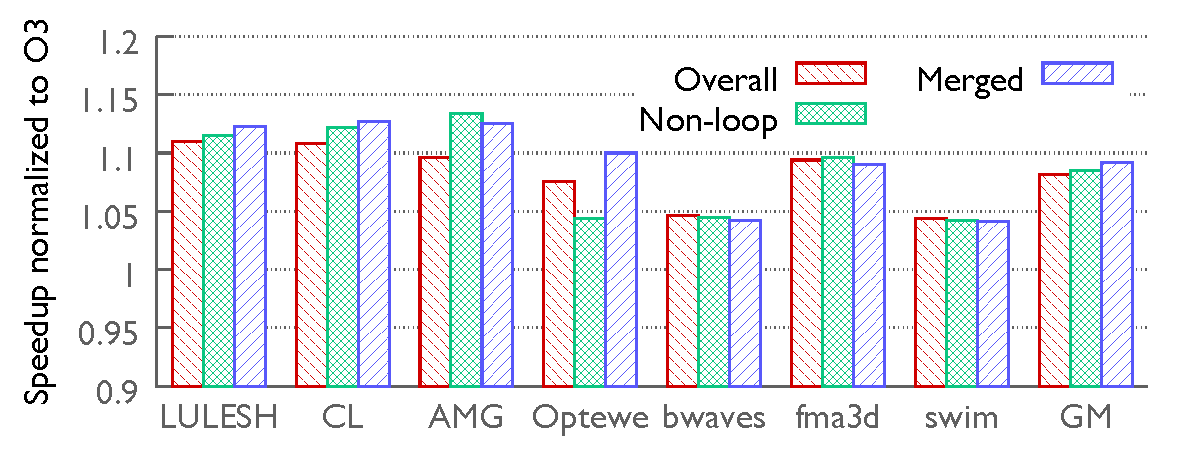
\includegraphics[scale=.4]
{gnuplot_temp/fc_broad.pdf}
\label{fig:sensitivityBroadwell}}
\vspace{-2mm}
\caption{Non-loop CV metrics: use of both derived non-loop runtime and overall runtime
metrics result in better performance.}
\label{fig:sensitivity}
\vspace{-4mm}
\end{figure}

These observations motivated us to combine the strength of the two metrics
(\emph{Non-loop} and \emph{Overall}) into one (denoted as
\emph{Merged} in \Cref{fig:sensitivity}), which concatenates the
top-30 best non-loop CVs from both \emph{Non-loop} and \emph{Overall}.
The concatenation results in 60 CVs for non-loop code, whereas only
the top-30 per-loop CVs are used for each hot loop.  Results in
\Cref{fig:sensitivity} show that \emph{Merged} delivers performance that
is either higher or close to the performance of \emph{Non-loop} and \emph{Overall}.  The reason for
this is that performant non-loop code CVs, which appear in both
\emph{Non-loop} and \emph{Overall} and are more likely to have a
positive performance impact, appear twice in \emph{Merged} and have a
higher probability of being used. Hence, in the remaining sections, we use
CFR to denote \emph{Merged} CFR.




\begin{figure*}
\subfloat[Part 1][Normalized speedups on AMD Opteron]
{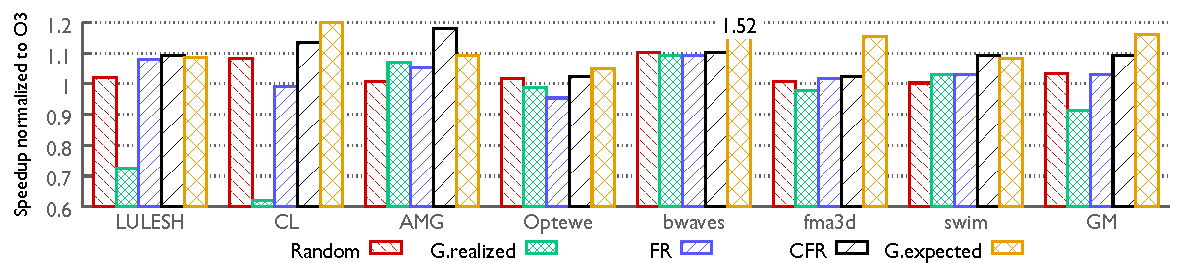
\includegraphics[width=\linewidth]
{gnuplot_temp/opteron.pdf}
\label{fig:ro}}
\vspace{-1em}
\subfloat[Part 1][Normalized speedups on Intel Sandy Bridge]
{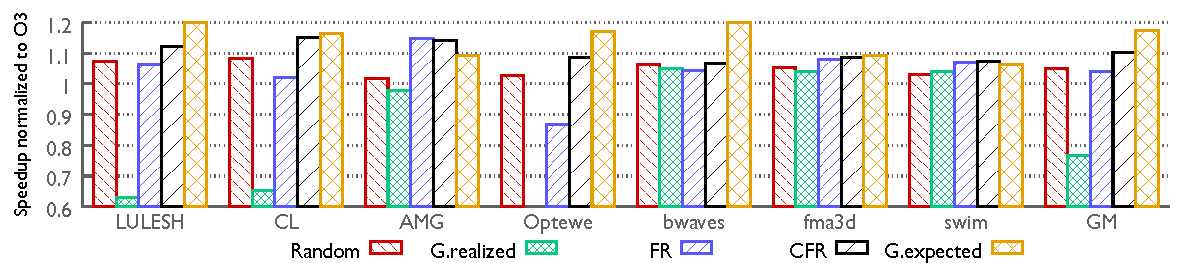
\includegraphics[width=\linewidth]
{gnuplot_temp/sandy.pdf}
\label{fig:rs}}
\vspace{-1em}
\subfloat[Part 1][Normalized speedups on Intel Broadwell]
{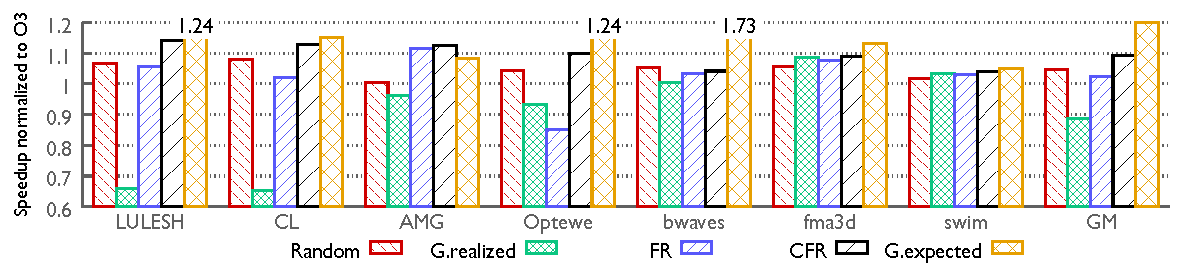
\includegraphics[width=\linewidth]
{gnuplot_temp/broad.pdf}
\label{fig:rb}}
%\vspace{-2mm}
\caption{CFR outperforms other methods for most cases: geometric mean of
speedups relative to the O3 baseline are 9.2\%, 10.3\%, and 9.4\% on
Opteron, Sandy Bridge, and Broadwell, respectively.}
\label{fig:results}
%\vspace{-2mm}
\end{figure*}


%results

%Caliper instrumentation usually incurs less than 5\% overhead.
% However, the overhead can be up to 30\% for Intel KNL many-core
% architecture due to high synchronization overhead.  Such high
% measurement overhead would dominate Caliper-based timing
% information, which makes CFR more important because its re-sampling
% and multiple-point evaluation can tolerate more measurement errors.
% However, we found even though non-loop code runtime is usually much
% smaller than total runtime of hot loops, its CVs plays a vital role
% in performance of the final binary.
\begin{comment}
\begin{figure}
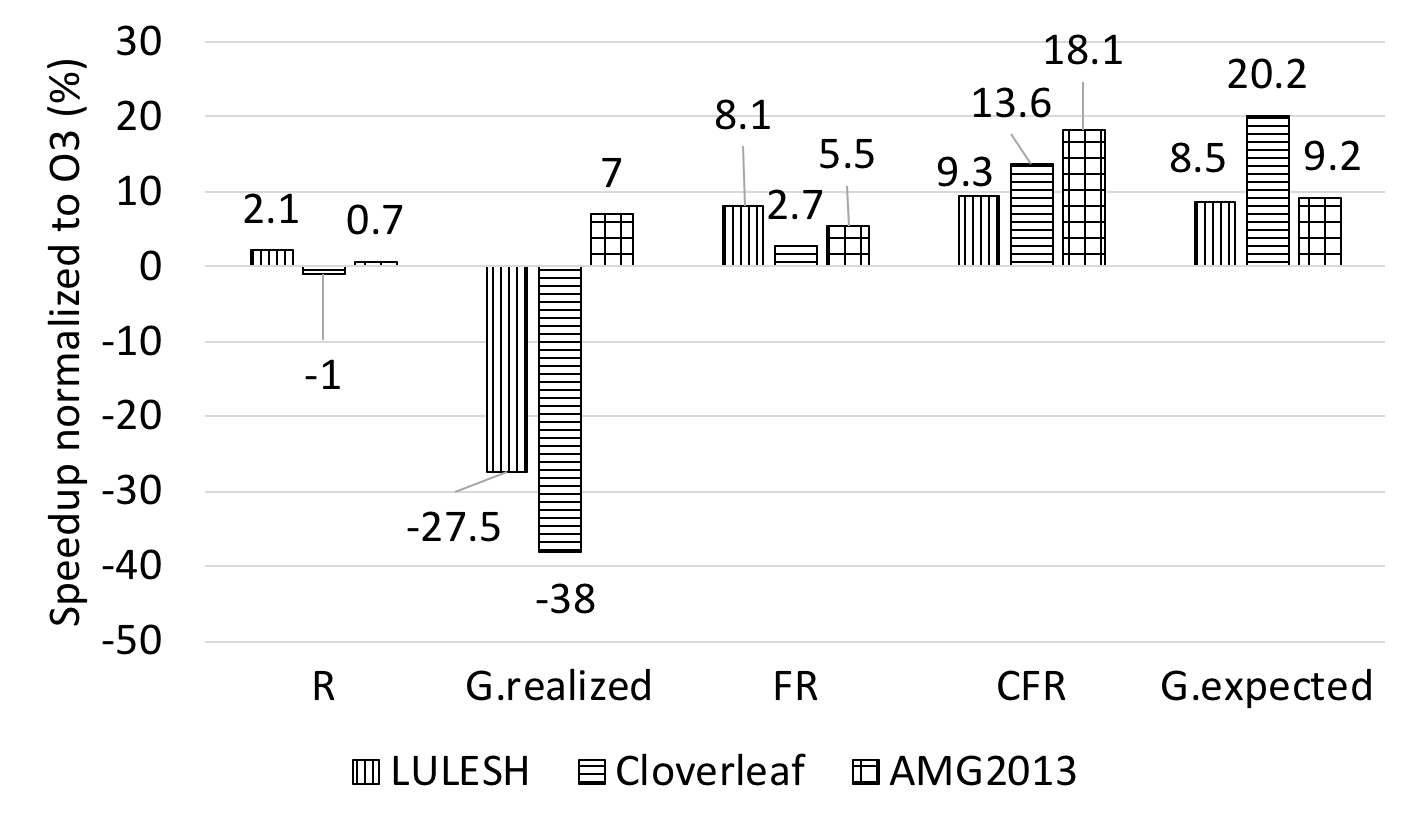
\includegraphics[width=\linewidth]{figures/speedup_opteron}
\caption{Normalized Speedup for Lulesh, Cloverleaf and AMG on AMD Opteron}
\label{fig:ro}

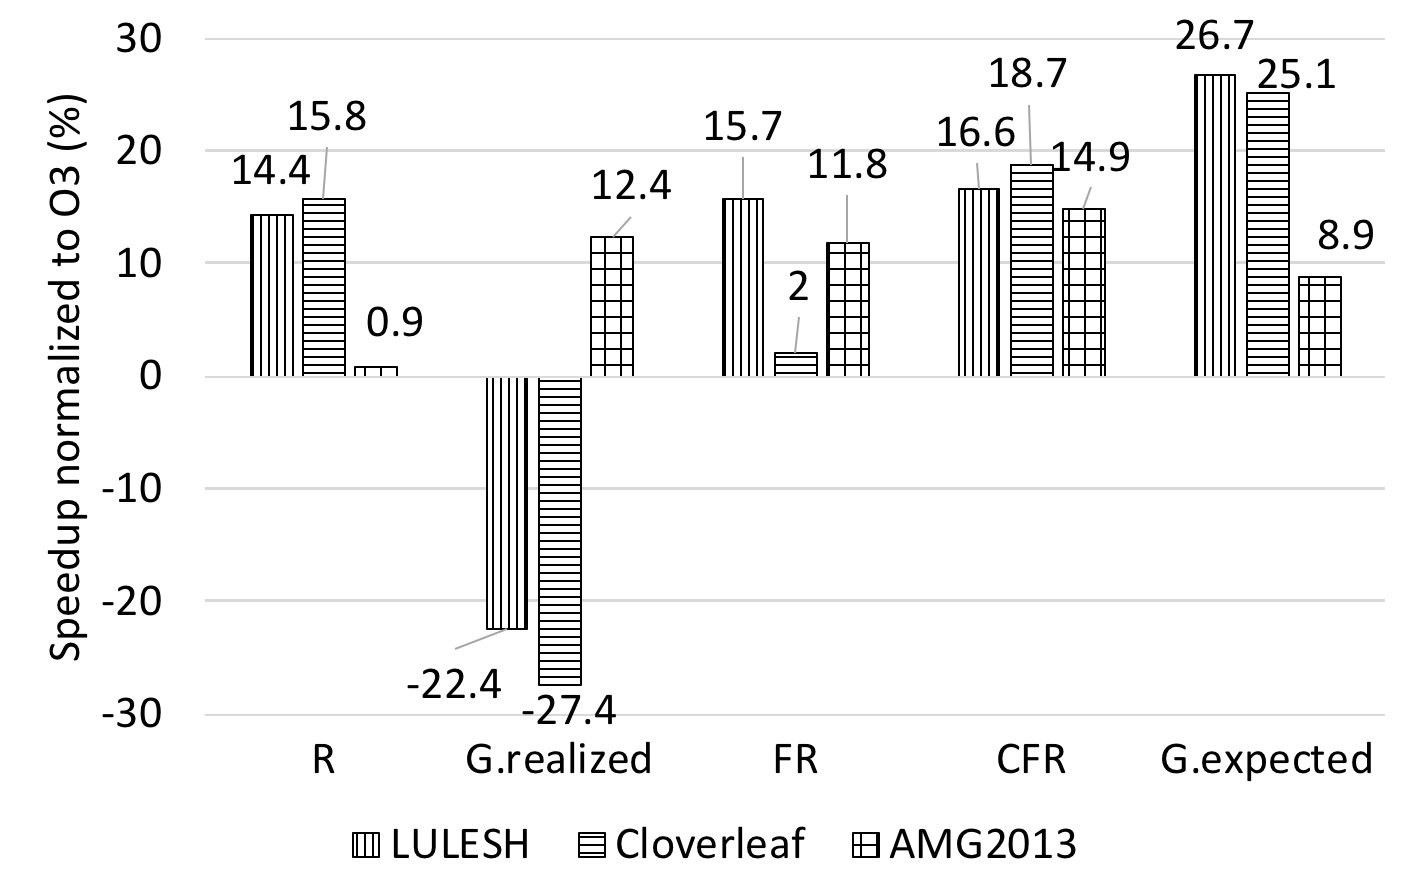
\includegraphics[width=\linewidth]{figures/speedup_sandy}
\caption{Normalized Speedup for Lulesh, Cloverleaf and AMG on Intel Sandy Bridge}
\label{fig:rs}

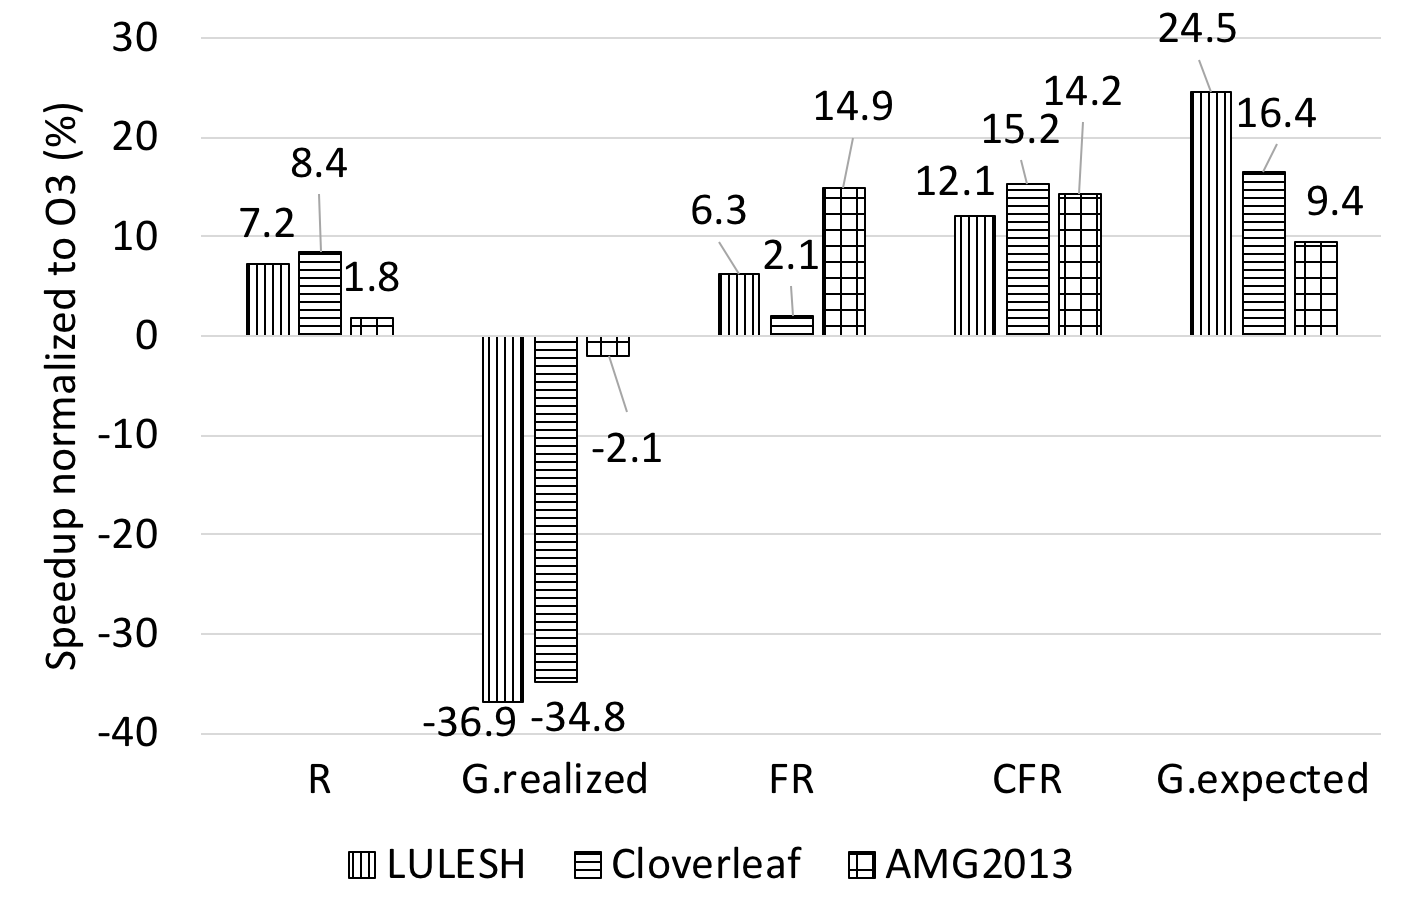
\includegraphics[width=\linewidth]
{figures/speedup_broadwell}
\caption{Normalized Speedup for Lulesh, Cloverleaf and AMG on Intel Broadwell}
\label{fig:rb}
\end{figure}
\end{comment}



\begin{comment}
\begin{figure}
\includegraphics[width=\linewidth]
{figures/overall}
\caption{Normalized Speedups on AMD Opteron}
\label{fig:arch}

\includegraphics[width=\linewidth]
{figures/overall}
\caption{Normalized Speedups on Intel Sandy Bridge}
\label{fig:arch}

\includegraphics[width=\linewidth]
{figures/overall}
\caption{Normalized speedups on Intel Broadwell. G.realized is the
  actual speedup of Greedy algorithm while G.expected is the expected
  speedup of Greedy algorithm, calculated by summing up the best
  per-loop run times. FR and CFR are the two fine-grained search
  algorithms proposed by us, applied on the benchmarks with their hot
  loops outlined and without Caliper instrumentation; R is random
  search on per-program granularity, with the original unmodified
  benchmarks. }
\label{fig:arch}
\end{figure}
\end{comment}

%\begin{figure*}
%\includegraphics[width=\linewidth]
%{figures/overall}
%\caption{Normalized speedups on Intel Sandy Bridge}
%\label{fig:arch}
%\end{figure*}

%\begin{figure*}

%\end{figure*}

\subsection{Overall Performance Comparison} \label{overallResults}

Performance results for our benchmarks on the three
architectures are shown in \Cref{fig:results}. In this figure, R is coarse-grained
random search (\Cref{fig:csr}) for the original unmodified benchmarks,
FR (\Cref{alg:fr}) and CFR (\Cref{alg:cfr}) are the two fine-grained search
algorithms proposed by us, G.realized is the observed speedup of
the Greedy algorithm (\Cref{alg:greedy}), and G.expected is the
theoretical expected speedup of the Greedy algorithm calculated by
summing up the best per-loop and non-loop runtimes, which serves as
an analytical upper bound. FR, CFR, G.realized, and G.expected are all
applied on the benchmarks with their hot loops outlined and without Caliper
instrumentation.
%with detailed performance statistics presented in \Cref{table:stdO,table:stdS,table:stdB}.
From these results, we make the following observations.

\vspace{.25em}
\noindent 1) CFR provides the best performing executables for most
scenarios across benchmarks and architectures. It provides 9.2\%,
10.3\%, 9.4\% geometric mean speedups for Opteron, Sandy
Bridge and Broadwell, respectively.  It also achieves the best case
improvement of 18.1\% for AMG on AMD Opteron (see \Cref{fig:ro}) in
comparison to the O3 baseline.  In contrast, the performance
improvement due to R is only 3.4\%, 5.0\%, 4.6\% on the same
respective architectures.  In certain cases, R does not improve performance at all
while CFR does much better, e.g., for AMG on Sandy Bridge and
Broadwell.
% The gap is less on KNL, which may be due to misleading of high
% measurement error for runtimes.  Note that even though loop
% outlining incurs 22.5\% slowdown for LULESH, compared to O3
% baseline, CFR still performs 2.8\% better than R, which is already
% 37.7\% better than the baseline.

\vspace{.25em}
\noindent 2) G.realized results in significant slowdowns for many benchmark and
architecture combinations.  Although it improves performance of AMG on
Opteron and Sandy Bridge, the improvement is still inferior to that of
CFR.

\vspace{.25em}
\noindent 3) FR's performance is inferior to CFR and has high
variance.  For example, it achieves less than a 3\% improvement for
Cloverleaf on Opteron, Sandy Bridge and Broadwell, while CFR achieves
13.6\%, 15.2\% and 12.7\%, respectively.
%Even worse, it degrades Cloverleaf performance by 25.8\% on KNL.

The above comparison between R and CFR confirms our hypothesis that
fine-grained per-loop compilation can improve
program performance beyond that of a traditional per-program compilation model.
A comparison with FR indicates that the \toolname
approach of flag selection based on observed per-loop timings is
critical for performance improvement.  Finally, poor results for G.realized indicate
that greedily picking the best CVs for each hot-loop and non-loop code
is not sufficient. %Instead, CFR's multi-step, profile-guided approach
%is needed to get higher performance.
\vspace{-2mm}
\subsection{Comparison to the State-of-the-art} \label{beatPGO}

To meet the objective of compiler flag selection for each hot loop and
thus specialize compilation for a specific application, several prior
search-based and machine learning-based approaches exist.  As a
search-based approach, FuncyTuner optimizes each new program by
searching the COS for performant CVs from scratch.  The
state-of-the-art search algorithm in~\cite{cere} performs a
fine-grained flag selection for hot code regions and generates the
final executable in a greedy fashion, similar to G.realized in our
work.  Our results in \Cref{fig:results} show that
this degrades performance for several benchmarks for the Intel compiler tool chain.

COBAYN~\cite{cobayn}, a state-of-the-art machine
learning-based approach, infers performant CVs for a new program by
extracting static and dynamic program features and providing them as inputs to a
pre-trained Bayesian network.  To compare FuncyTuner with COBAYN, we
first train COBAYN on Intel Broadwell with cBench~\cite{cbench}.
Specifically, we select the top 100 performant CVs out of 1000 random
CV samples for each cBench application to extract their static and
dynamic features with Milepost-gcc~\cite{milepostgcc} and
Mica~\cite{mica}, respectively.  We then train three models,
{\em static, dynamic, and hybrid}, using static features, dynamic features
and all features, respectively.  Since COBAYN can only
perform inferences on binary compiler flags, we turn each multi-valued
ICC flag into a binary one by allowing it to have two values.  Then,
we use each of the three COBAYN models to generate 1000 CVs to compile
1000 code variants. The fastest code variant is considered as the
result of each model.  This comparison is fair, since both FuncyTuner
and COBAYN pick the best variant using information derived from data on 1000  variants.
\begin{figure*}
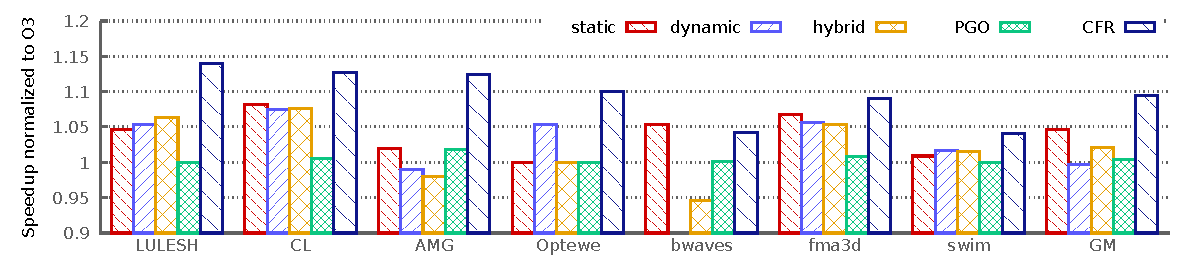
\includegraphics[width=\linewidth]{gnuplot_temp/pgo.pdf}
\vspace{-6mm}
\caption{FuncyTuner provides better performance than all variants of COBAYN(static, dynamic, hybrid) and PGO.}
\label{fig:pgo}
\vspace{-2mm}
\end{figure*}
%PGO results will be put here, together w/ COBAYN
%Figure needs to be redrawn
Both search-based approaches, FuncyTuner and COBAYN (and machine-learning techniques in general), take runtimes of different code variants as inputs.  However, runtimes are
only one of many program performance profile considerations.  In fact,
Intel compilers support built-in profile-guided
optimization~\cite{pgo} (PGO), which utilizes an instrumentation run
of a target program to collect profile information, such as loop trip
counts and indirect function call targets.  Therefore, the comparison
to PGO offers a perspective to evaluate the trade-off between benefits
and complexities for all approaches.  For a fair comparison, we use
"-qopenmp -fp-model source -prof-gen -prof-dir/app" for an
instrumented compilation (see recommendations for PGO in Intel's
compiler optimization manual) and then run the programs with tuning
inputs in \Cref{settings}.  Afterward, the programs are recompiled
with ``-O3 -qopenmp -fp-model source -prof-use -prof-dir/app''.

\begin{comment}
\begin{figure*}
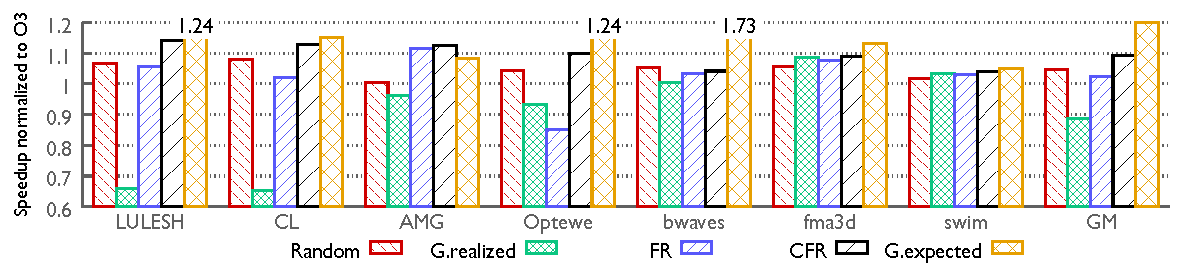
\includegraphics[width=\linewidth]{gnuplot_temp/broad.pdf}
\caption{Normalized Speedup for Lulesh, Cloverleaf and AMG on AMD Opteron}
\label{fig:ro}
\end{figure*}
\end{comment}

\begin{comment}
\begin{figure}
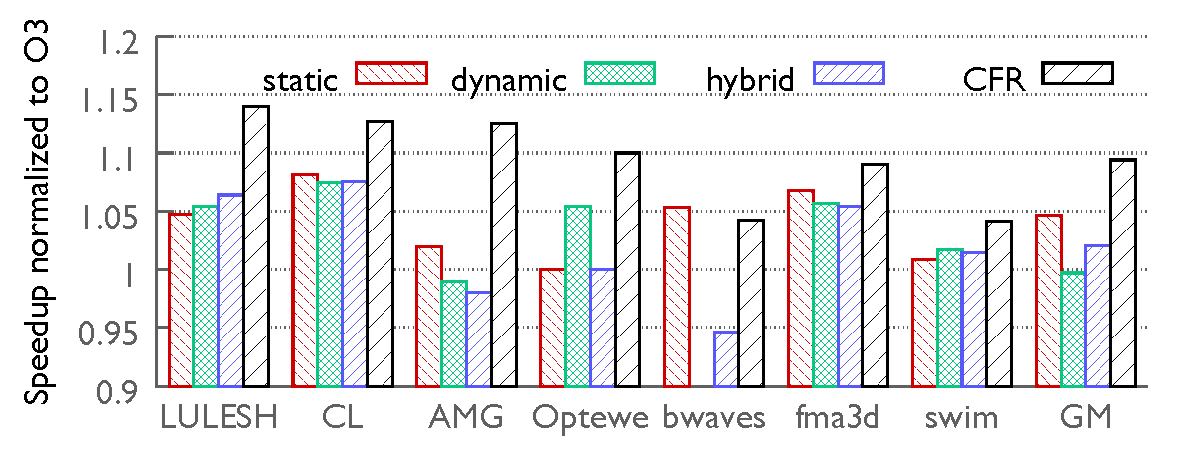
\includegraphics[width=\linewidth]{gnuplot_temp/cobayn_compare.pdf}
\caption{FuncyTuner provides better performance than all variants of
    COBAYN (static, dynamic, hybrid).}
\label{fig:cobayn}
\end{figure}
\end{comment}

Results are shown in \Cref{fig:pgo}. Specifically, we make the following observations:

\noindent (1) COBAYN's static and hybrid models perform
4.6\% and 2.1\% (geometric mean) better than the O3 baseline, respectively,
while COBAYN's dynamic model is worse than the O3 baseline.
In contrast, FuncyTuner CFR improves performance by 9.4\% beyond the O3 baseline and outperforms COBAYN significantly.
  The
performance of COBAYN's static model is consistent with the findings
in the work that proposed COBAYN~\cite{cobayn} and other previous
research~\cite{1611549,Cavazos:2007:RSG:1251974.1252540,FursinMGL15}.
These related works also show that
a machine learning-based approach is able to reduce search overhead but
does not perform better than traditional random search ("Random" in our
paper) when the sample size is sufficiently large, e.g., 1000 samples.
The poor performance of COBAYN's dynamic and hybrid models may be
attributed to limited dynamic features, since MICA~\cite{mica} only
works with serial code while our target benchmarks are parallel.
% We also want to point out that FuncyTuner has little overhead to be
% ported onto different machines, while the re-training overhead can
% be prohibitively high for COBAYN.  As an example, extracting dynamic
% features for cBench takes around 2 days on a 16-node Broadwell
% cluster.

\noindent (2) PGO result in only minor performance improvements
relative to O3 and is inferior to \toolname CFR.  While PGO is 1.8\%
better than O3 for AMG, it shows little improvement on six other
programs.  In fact, PGO instrumentation runs fail for LULESH and
Optewe. 
%, and we consider its performance identical to O3. --> Frank:
%Dont say that, and don't report something you did nto measure!

In brief, \toolname delivers significantly better performance than
state-of-the-art techniques on our modern scientific simulation codes.
It only relies on Caliper light-weight source-code level
instrumentation \cite{caliper}, entailing much less engineering
complexities than both COBAYN and PGO.  Such simplicity is extremely
noticeable when one considers the fact that Intel compilers are
industry-quality production compilers and tuned for several decades,
and COBAYN depends on a variety of large tools, such as Milepost GCC
\cite{milepostgcc} and Mica.  Nevertheless, their performance is
inferior to \toolname and their robustness is limited.

\iffalse
\begin{figure}
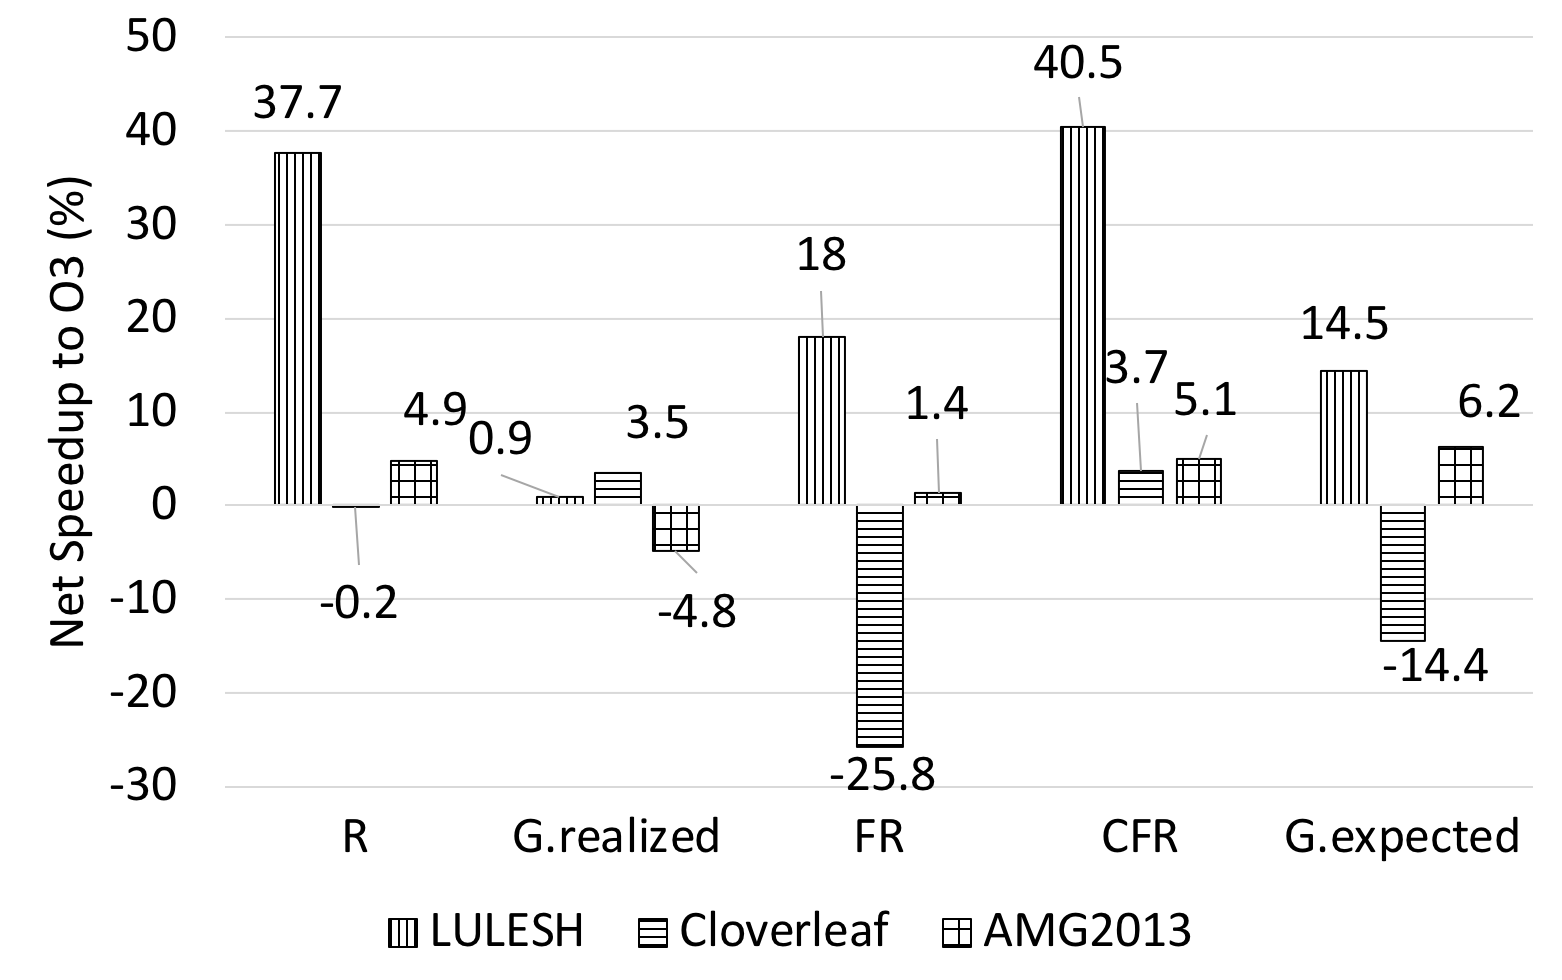
\includegraphics[width=\linewidth]{figures/speedup_knl}
\caption{Net Speedup for Lulesh, Cloverleaf and AMG2013 on
    Intel Knights Landing}
\label{fig:rk}
\end{figure}
\fi

\begin{comment}
\begin {table}
%\nocaptionrule
\caption{Performance Statistics on Intel Broadwell}
\label{table:stdB}
%\vspace{2pt}
\centering
\resizebox{\columnwidth}{!}{%
\begin{tabular}{l|l|l|l|l|l|l }
\hline
%  & \\
\multirow{2}{*}{\textbf{Algorithm}} &  \multicolumn{2}{c|}{\textbf{Lulesh}} & \multicolumn{2}{c|}{\textbf{Cloverleaf}} & \multicolumn{2}{c}{\textbf{AMG}} \\
\cline{2-7}
 & \textbf{Mean} & \textbf{stdev} & \textbf{Mean} & \textbf{stdev} & \textbf{Mean} & \textbf{stdev} \\
\hline
%  & \\
G.expected & 10.9   & N/A & 5   & N/A & 11.8  & N/A\\
\hline
G.realized & 21.52 & 1.4 & 8.92 & 0.29 & 13.19 & 0.65 \\
\hline
O3.origin & 13.57 & 0.04 & 5.82 & 0.07 & 12.91 & 0.29 \\
\hline
O3.caliper & 13.91 & 0.05 & 5.91 & 0.08 & 13.4 & 0.48\\
\hline
O3.outlined & 13.82 & 0.04 & 5.79 & 0.06 & 12.97 & 0.48\\
\hline
R & 12.66 & 0.07 & 5.37 & 0.04 & 12.68 & 0.1 \\
\hline
FR & 12.76 & 0.07 & 5.7 & 0.05 &11.24 & 0.06\\
\hline
CFR & 12.11 & 0.42 & 5.05 & 0.04 & 11.3 & 0.08\\
\hline
\end{tabular}
}
\end {table}

\begin {table}
%\nocaptionrule
\caption{Performance Statistics on Intel Sandy Bridge}
\label{table:stdS}
%\vspace{2pt}
\centering
\resizebox{\columnwidth}{!}{%
\begin{tabular}{l|l|l|l|l|l|l }
\hline
%  & \\
\multirow{2}{*}{\textbf{Algorithm}} &  \multicolumn{2}{c|}{\textbf{Lulesh}} & \multicolumn{2}{c|}{\textbf{Cloverleaf}} & \multicolumn{2}{c}{\textbf{AMG}} \\
\cline{2-7}
 & \textbf{Mean} & \textbf{stdev} & \textbf{Mean} & \textbf{stdev} & \textbf{Mean} & \textbf{stdev} \\
\hline
%  & \\
G.expected & 5.7  & N/A & 3.7 & N/A & 6.1 & N/A\\
\hline
G.realized & 9.3 & 0.16 & 6.38 & 0.22 & 5.91 & 0.03 \\
\hline
O3.origin & 7.22 & 0.05 & 4.63 & 0.01 & 6.64 & 0.17 \\
\hline
O3.caliper & 8.0 & 0.05 & 4.76 & 0.04 & 7.4 & 0.3\\
\hline
O3.outlined & 7.39 & 0.08 & 4.65 & 0.03 & 6.66 & 0.13\\
\hline
R & 6.31 & 0.17 & 4 & 0.02 & 6.58 & 0.18 \\
\hline
FR & 6.24 & 0.12 & 4.54 & 0.03 &5.94 & 0.04\\
\hline
CFR & 6.19 & 0.18 & 3.9 & 0.01 & 5.78 & 0.02\\
\hline
\end{tabular}
}
\end {table}

\begin {table}
%\nocaptionrule
\caption{Performance Statistics on AMD Opteron}
\label{table:stdO}
%\vspace{2pt}
\centering
\resizebox{\columnwidth}{!}{%
\begin{tabular}{l|l|l|l|l|l|l }
\hline
%  & \\
\multirow{2}{*}{\textbf{Algorithm}} &  \multicolumn{2}{c|}{\textbf{Lulesh}} & \multicolumn{2}{c|}{\textbf{Cloverleaf}} & \multicolumn{2}{c}{\textbf{AMG}} \\
\cline{2-7}
 & \textbf{Mean} & \textbf{stdev} & \textbf{Mean} & \textbf{stdev} & \textbf{Mean} & \textbf{stdev} \\
\hline
%  & \\
G.expected & 9.7  & N/A & 5.73 & N/A & 9.4 & N/A\\
\hline
G.realized & 14.52 & 0.37 & 11.01 & 0.15 & 9.6 & 0.07 \\
\hline
O3.origin & 11.1 & 0.08 & 6.88 & 0.16 & 10.27 & 0.25 \\
\hline
O3.caliper & 11.05 & 0.05 & 7.38 & 0.09 & 10.99 & 0.62\\
\hline
O3.outlined & 10.84 & 0.03 & 6.89 & 0.14 & 10.13 & 0.25\\
\hline
R.origin & 10.87 & 0.08 & 6.96 & 0.12 & 10.19 & 0.37 \\
\hline
FR & 10.27 & 0.05 & 6.7 & 0.07 & 9.73 & 0.92 \\
\hline
CFR & 10.16 & 0.05 & 6.06 & 0.08 & 8.7 & 0.27\\
\hline
\end{tabular}
}
\end {table}
\end{comment}

\iffalse
\begin {table}[!htb]
%\nocaptionrule
\caption{\textbf{Performance Statistics on Intel KNL}}
\label{table:stdK}
%\vspace{2pt}
\centering
\resizebox{\columnwidth}{!}{%
\begin{tabular}{l|l|l|l|l|l|l }
\hline
%  & \\
\multirow{2}{*}{\textbf{Algorithm}} &  \multicolumn{2}{c|}{\textbf{Lulesh}} & \multicolumn{2}{c|}{\textbf{Cloverleaf}} & \multicolumn{2}{c}{\textbf{AMG}} \\
\cline{2-7}
 & \textbf{Mean} & \textbf{stdev} & \textbf{Mean} & \textbf{stdev} & \textbf{Mean} & \textbf{stdev} \\
\hline
%  & \\
G.expected & 6  & N/A & 6.2 & N/A & 8.74 & N/A\\
\hline
G.realized & 6.81 & 0.01 & 5.13 & 0.01 & 9.75 & 0.02 \\
\hline
O3.origin & 6.87 & 0.11 & 5.31 & 0.01 & 9.28 & 0.01 \\
\hline
O3.caliper & 9.77 & 0.04 & 6.48 & 0.01 & 9.64 & 0.03\\
\hline
O3.outlined & 8.87 & 0.02 & 5.33 & 0.01 & 9.29 & 0.05\\
\hline
R & 4.99 & 0.01 & 5.32 & 0.01 & 8.85 & 0.01 \\
\hline
FR & 5.82 & 0.01 & 7.16 & 0.02 &9.15 & 0.02\\
\hline
CFR & 4.89 & 0.01 & 5.12 & 0.01 & 8.83 & 0.03\\
\hline
\end{tabular}
}
\end {table}
\fi

\subsection{Impact Of Different Inputs} \label{inputsensitivity}
\begin{figure}
\centering
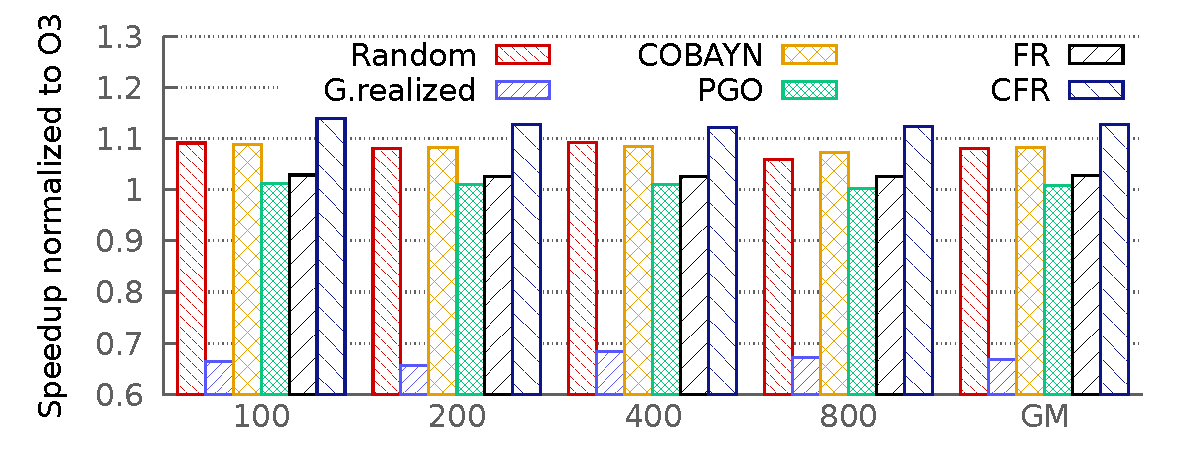
\includegraphics[width=0.6\textwidth]{gnuplot_temp/scale_CL.pdf}
%\vspace{-5mm}
\caption{For Cloverleaf on Broadwell, FuncyTuner CFR provides stable performance benefit than all others while scaling from 100 to 800 time-steps.}
\label{fig:cl}
%\vspace{-5mm}
\end{figure}

\begin{figure*}
\subfloat[Part 1][Normalized speedups for small inputs]
{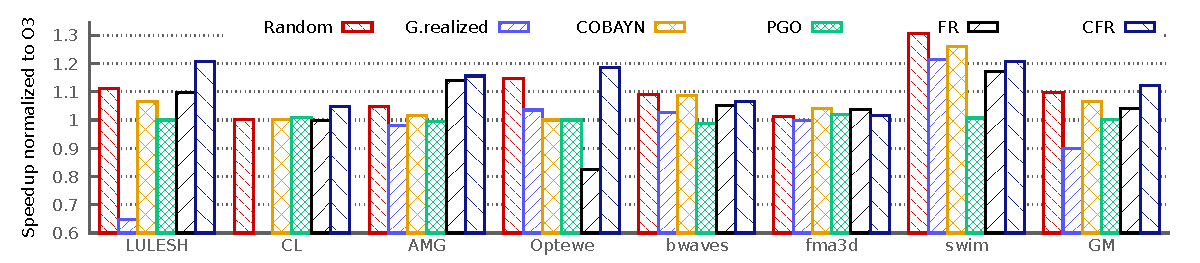
\includegraphics[width=\linewidth]
{gnuplot_temp/small.pdf}
\label{fig:small}}
\vspace{-1em}
\subfloat[Part 1][Normalized speedups for large inputs]
{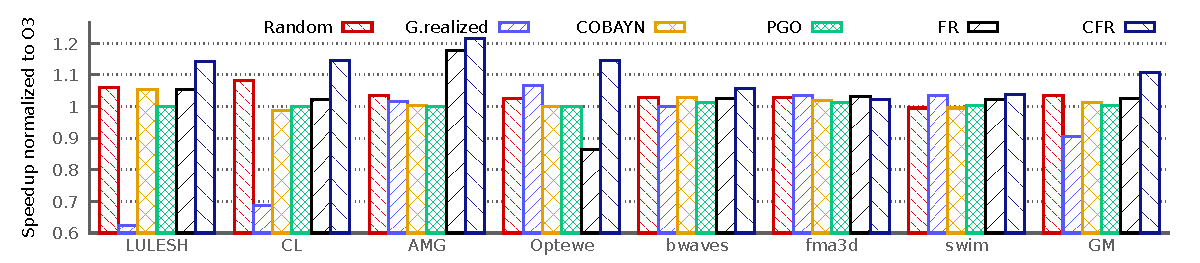
\includegraphics[width=\linewidth]
{gnuplot_temp/large.pdf}
\label{fig:large}}
\vspace{-2mm}
\caption{CFR shows little performance sensitivity on small and large inputs with geometric mean of speedups relative to the O3 baseline 12.3\% and 10.7\% respectively.}
\vspace{-4mm}
\label{fig:sensitivity}
\end{figure*}
The over-arching goal of our work is to auto-tune large scientific
simulation codes with a given input.  Such inputs capture the sizes of
work sets in practice, hence, their performance generalizes to other
inputs as we will show, e.g., for inputs with the same work-set size
but different simulation time-steps. This is shown in
\Cref{fig:cl} for Cloverleaf on Broadwell by varying number of
time-steps as part of the input.
\begin{comment}
\begin {table}[t]
%\nocaptionrule
\caption{Small and large inputs. Format}
%\vspace{2pt}
\centering
{\footnotesize
\label{table:apps}
\begin{tabular}{ p{1.7cm}p{2.0cm}p{1.7cm}}
%\hline
%  & \\
\textbf{Name} & \textbf{Small} & \textbf{Large}\\
\hline
AMG & 20 & 30 \\ \hline
LULESH & 180& 250\\ \hline
Cloverleaf (CL) & 1000 & 4000\\ \hline
351.bwaves & test & ref \\ \hline
362.fma3d & test & ref \\ \hline
363.swim & test & ref \\ \hline
Optewe & 384& 768\\ \hline
\end{tabular}
}
\end {table}
\end{comment}

\begin{comment}
\begin {table}[t]
%\nocaptionrule
\caption{List of benchmarks. LOC: lines of source code.}
%\vspace{2pt}
\centering
{\footnotesize
\label{table:apps}
\begin{tabular}{ p{1.7cm}p{2.0cm}p{3.4cm}}
%\hline
%  & \\
\textbf{Name} & \textbf{Small} & \textbf{Large}\\
\hline
AMG & 20 & 30 \\ \hline
LULESH & 180,10 & 250,5 \\ \hline
Cloverleaf (CL) & (1000,300) & (4000,10)\\ \hline
351.bwaves & test (5, 150) & ref (160, 10) \\ \hline
362.fma3d & test (1, 8000) & ref (END=1.5E-4, END=1.5E-6) \\ \hline
363.swim & test (10, 20000) & ref (3000, 50) \\ \hline
Optewe & 384, 15 & 768, 1\\ \hline
\end{tabular}
}
\end {table}
\end{comment}

Inputs with different work-set sizes are addressed as follows.  We
experimented on Broadwell with two sets of inputs that have different
input sizes from those in \Cref{settings}. For 351.bwaves, 362.fma3d,
and 363.swim, we use ``test'' and ``ref'' as their small and large
inputs, respectively. For LULESH, AMG, Cloverleaf, Optewe, their small
input sizes are 180, 20, 1000, 384, respectively, while their large
input sizes are 250, 30, 4000, 768, respectively.  As shown in
\Cref{fig:sensitivity}, we observe little sensitivity for these small
and large inputs, except that for 351.swim \toolname CFR does not
perform as well as the other three approaches for its small
input. Nonetheless, CFR for 351.swim is still 20.6\% better than PGO and the
O3 baseline.  We attribute such performance to the fact that the
``test'' input is so small that each time-step takes less than .01
seconds, which significantly differs from the performance profile of its
tuning input.
%In fact, the instrumentation overhead is 41.2\% high of its O3 baseline. 
However, such a small input rarely exists in practice and is not our
primary focus.

%{\bf Why is the following commented out? Check the latex source! Is
%  this intentional?} Answer by Tao {Yes. The commented one was the first draft I had, not usable anymore.}
\begin{comment}
In our experimental settings, we verify that this is true with O3 baseline when we conduct the input size reduction.
We further verify this property on Intel Broadwell with inputs different from the tuning inputs.
%
These inputs are selected according to the following two
guidelines: 1) Increase the time-steps for tuning-inputs, and 2) increase
the input scales.

Our experiments show that on the inputs of interest to scientific
simulation codes, there is little input sensitivity and the tuning
performance benefits can generalizes beyond the training inputs.
\end{comment}
%A prior work \cite{Chen:2010:EIO:1806596.1806647} by Chen et al. validates that search-based tuning has limited input sensitivity across 1000 inputs on their benchmark suite.
%To the best of our knowledge, there is no guideline to select inputs so that they will capture different work sets automatically.


\vspace{-1ex}
\subsection{Deep Dive: Cloverleaf On Broadwell} \label{case-study}

% Furthermore, CFR evaluates 1000 MCVs re-sampled from the per-loop
% compressed CV sample space in contrast to G, which only evaluates
% one MCV. This enables CFR to learn from diverse interactions among
% different CVs and compilation modules to obtain higher performing
% executables.  To gain further insights, we conduct an in-depth case
% study for Cloverleaf on Intel Broadwell.  motivation

\subsubsection{\textbf{Design}}

Broadly speaking, CFR utilizes per-loop runtime
information to direct the fine-grained search towards better
performing CVs.  Insights about the performance characteristics of
different algorithms compared in this paper can be useful for further
improving program performance.  Specifically, we want to answer the
following two questions:
%Thus, we carry out a case study to answer the following two questions:
\begin{itemize}
\item \textbf{$Q_1$}: Why does G.realized often introduce slowdowns
  while expected to have performance improvements?
\item \textbf{$Q_2$}: Why does CFR perform better than others?
\end{itemize}

% approach To this end, we perform an in-depth analysis of Cloverleaf
% on Intel Broadwell.
To this end, we select Cloverleaf to perform an in-depth case study on
Intel Broadwell due to the following considerations: first, its
non-loop code is written in Fortran, and hot loops are in C.  This may
provide more challenges and opportunities for ICC's inter-procedural
optimizations (IPO).  Second, its hot loops have simple source code
structures, e.g., they neither feature control flow nor deep loop
nests, thus presenting opportunities for ICC to perform optimizations
related to loop unrolling and vectorization, which often have a
significant impact on program performance.
% and are friendly for manual inspection of generated code to
% understand how they have been performed.
Five hot loops of Cloverleaf are selected since they have
comparatively high per-loop runtime ratios (see \Cref{table:study},
others are less than 3.0\%) and were found to produce large
performance differences (see \Cref{fig:case}) across different
tuning algorithms.
%, which provides more opportunities to interpret them with Likwid fine-grained profiling data~\cite{likwid}.

%more about approach: greedy reduction
Since each CV has more than 30 flags, it is difficult to identify
performance-critical flags in the best CVs chosen by different algorithms.
We use a greedy
algorithm to eliminate the flags that have low impact on the
program runtime.  The algorithm tries to eliminate one
flag for a specified loop CV (\emph{focused CV}) while
keeping all other CVs intact.  If excluding a flag from \emph{focused
  CV} does not degrade program performance, the flag is removed;
otherwise, it is kept intact.  This process is performed iteratively until no more
flags of \emph{focused CV} can be eliminated.  We consider the remaining flags in
\emph{focused CV} as the critical ones for the given loop.
Note that we only consider the static COBAYN model, because it is
superior to its dynamic and hybrid counterparts for Cloverleaf.
% Let's denote the flag being considered as $F_c$
%
% If there is no performance degradation while excluding the flag under
% consideration from then After one iteration of evaluating flags of
% the given CV, it keeps all flags that contribute to performance
% improvements (i.e., if such a flags were to be removed, performance
% would drop).  without performance degradation, which guarantees that
% the reduced CVs produce a binary with similar runtime (within 1\%
% difference).  This enables us to reason which flags are critical for
% a compilation module of interest.

\begin {table}
%\nocaptionrule
  \caption{Critical flags for Cloverleaf. O3 is always included in the CV.}
  \vspace{-3mm}
\label{table:algs}
\small
\centering
\begin{tabular}{ l|l|l }
%\hline
%  & \\
\textbf{Algorithm} & \textbf{Loop} & \textbf{Flags} \\
\hline
R/COBAYN & all &-qopt-streaming-stores=always\\
 & &-no-ansi-alias -ipo -xCORE-AVX2 \\
\hline
CFR& dt & -no-vec\\
\hline
CFR& cell3 & none\\
\hline
CFR& cell7 & none\\
\hline
CFR& mom9 & -no-vec\\
\hline
G.realized & mom9 & none \\
\hline
\end{tabular}
\vspace{-4mm}
\end {table}


\subsubsection{\textbf{Observations}}

%results and observation
\Cref{fig:case} shows the per-loop normalized performance
improvement due to G.realized, R/COBAYN, CFR, and G.expected for the five Cloverleaf
hot loops on Broadwell.  After greedy
elimination, the COBAYN static model has the same critical flags as those
of R, and thus they share the same results.  \Cref{table:study} reveals which critical
optimizations, such as loop unrolling and vectorization, are exploited by
different algorithms in this case.
\begin{comment}

Unless explicitly mentioned, there is no
loop unrolling.  Here, unroll2 and unroll3 indicate unroll twice and
three times, respectively.  There is no vectorization (scalar) by
default.  Broadwell has a 256-bit width SIMD unit.  With
``-xCORE-AVX2'', ICC can choose 128-bit or 256-bit SIMD instructions
for vectorization.  128-vec vectorizes a loop with 128-bit simd
instructions while 256-vec may use both 128-bit and 256-bit simd
instructions. \emph{RS} has register-spilling instructions.  \emph{IO}
means that instruction scheduling order is different from the one
without IO but with same notations, e.g., neither CFR nor G.realized
vectorizes Cloverleaf dt loop, but their generate code with different
instruction ordering.  \emph{IS} indicates that different instructions
are selected.  For example, both G.realized and R vectorizes loop
mom9, but instructions are different.
%, by inspecting the assembly code of binaries generated by them.
\end{comment}
We make the following observations:

\vspace{.25em}
\noindent (1) Vectorization is not always profitable. First, cell3
  and cell7 experience a 27.7\% and 13.6\% slowdown, respectively,
  when 256-bit vectorization is performed for R.  Other
  algorithms feature similar performance benefits, yet they do not
  vectorize.  Also, O3 uses 128-bit SIMD (single instruction multiple data) instructions.  Second, even though dt achieves a 34.8\%
  speedup with 256-bit vectorization, the performance improvement is
  still 12.8\% worse than a non-vectorized/scalar version. 
%
  Inspection of assembly code shows that there are many data permutations
  and mask operations to handle control flow divergence, which are
  known to degrade vectorization efficiency. Shorter loop trip counts
  caused by loop unrolling and OpenMP work sharing also
  contribute to the inferior performance of the vectorized loops.
\begin {table}
%\nocaptionrule
\caption{Comparison of optimizations for 5 Cloverleaf
kernels on Broadwell. scalar: not vectorized; \{128,256\}-vec: vectorized with
\{128,256\}-bit SIMD; unroll\{2,3\}: unroll 2/3 times; IO: instruction reordering;
IS: instruction selection; RS: register spilling.
}
\vspace{-2mm}
\label{table:study}
%\vspace{2pt}
\centering
%\resizebox{\columnwidth}{!}{%
\begin{tabular}{l|l|l|l|l|l }
\hline
%  & \\
\multirow{2}{*}{\textbf{Algorithm}} &  \multicolumn{5}{c}{\textbf{Kernel, O3 runtime ratio \%}} \\
\cline{2-6}
 & \textbf{dt, 6.3} & \textbf{cell3, 2.9} & \textbf{cell7, 3.5} & \textbf{mom9, 3.5} &\textbf{acc,  4.2} \\
%  & 6.3 & 2.9 & 3.5 & 3.5 & 4.2  \\
\hline
G.realized & scalar, IO & scalar & scalar & 256-vec, unroll2 &256-vec, IS, IO\\
%&IO & & & unroll2 &IS, IO\\
\hline
G.expected & scalar, RS, IO & scalar & scalar & scalar, IS & 256-vec \\
% & &  &  & IS &  \\
\hline
O3.origin & scalar, unroll2 & scalar & scalar & 128-vec & scalar, unroll3\\
%&  & & & &\\
\hline
R (COBAYN static)& 256-vec & 256-vec & 256-vec & 256-vec, IS &256-vec, IS\\
% &  &  &  & IS &IS\\
\hline
CFR & scalar & scalar & scalar & scalar, IS& 256-vec\\
% &  &  &  & IS &\\
\hline
\end{tabular}
%}
\vspace{-4mm}
\end {table}

\vspace{.25em}
\noindent (2) G.realized performs worse than other algorithms.
With different per-loop CVs from those of G.expected, IPO decisions are subject to changes. For example, G.realized vectorizes mom9 with 256-bit AVX2 instructions and further unrolls the vectorized loop twice while G.expected does not. In contrast, \toolname CFR has more informed freedom to select non-conflicting CVs. e.g., it selects "-no-vec" for mom9 to avoid vectorization.
%since IPO can invalidate decisions made earlier by local per-loop  cost
%  models.  For example, G.realized vectorizes mom9 with 256-bit AVX2
%  instructions and further unrolls the vectorized loop twice while
%  G.expected does not.
%  In contrast, CFR alleviates the conflict that G.realized experiences with IPO by
%  sampling more CVs in $COS_{new}$ with Caliper's guidance.
%  In fact, CFR selects a CV which does not use IPO for mom9.
  
  %so that it is able to find out CVs which have fewer conflicts.
  %\textbf{(How does more sampling concretely alleviate this? What are
  %  the flag differences??? Too vague, could backfire. Can you verify
  %  that CFR does not include IPO in this case? If so, mention it here.)}

\vspace{.25em}
\noindent (3) Other optimizations, such as instruction scheduling (IO), register
  allocation (RS), loop unrolling (unroll), and instruction selection (IS), also
  matter, e.g., CFR and G.expected both choose not to
  vectorize mom9, but their difference in instruction selection
  results in better performance for CFR.
%  Moreover, instruction scheduling plays a critical role in acc's performance slowdowns for G.realized.

In summary, we observe that such findings are difficult to derive
manually for compiler writers while auto-tuning with \toolname CFR is
able to capitalize on them.

\section{Related Work} \label{related work}

% why do we need tuning?
% To achieve peak performance and power efficiency for scientific applications on today's HPC machines, it is necessary to tune various compile-time and runtime configurations.
%On one side, configurations such as compile-time optimizations, runtime library parameters, and architectural configurations, may have a significant impact \cite{iterativecompilation, Chen:2010:EIO:1806596.1806647, powerTuner, energyTuner, cluster2016, sc2017}.
%On the other side, settings effective for one program/machine combination may not achieve peak performance on another, and it is both tedious and challenging to manually find the best configuration \cite{sc04oliver}.
%To attain the best performance, it is vital to automate the space exploration in an efficient manner.

% overview
 The first order objective of compiler-based auto-tuning techniques \cite{Hall:2009:CRN:1461928.1461946,grandstrand:2004} is performance, while the second order objectives are code size, power draw, and energy consumption.
 We divide prior work into the following two categories

\vspace{.25em}
\noindent (1) Compiler flag selection techniques \cite{1611551,PanE06,iterativecompilation,Cavazos:2007:RSG:1251974.1252540, Pan:2008:taco, cere, cern2012,Chen:2010:EIO:1806596.1806647, Vaswani:2007:MSE:1251974.1252536, Kulkarni:2004:FSE:996841.996863, 4625477}:
given a set of compiler flags, the objective is to determine the combination that generates the most performant executable on a given architecture.
Our work and many related papers \cite{Chen:2010:EIO:1806596.1806647, cere,PanE06,Pan:2008:taco} belong to this category.
\cite{Pan:2008:taco, cere} also take a fine-grained per-region approach.
They select the best code variant for each region in a greedy fashion without
considering interactions among different code variants; this is is effective for
their case studies but results in  worse performance than random search
for OpenMP-based scientific applications.
To reduce the overhead of search-based approaches, researchers have also proposed
schemes based on machine learning techniques \cite {1611549, Cavazos:2007:RSG:1251974.1252540, cobayn}.
As the state-of-the-art, COBAYN \cite{cobayn} infers good compile flags for a new program by representing them as static/dynamic features to a pre-trained Bayesian network.
Our experimentation shows that FuncyTuner outperforms COBAYN for Intel compiler
while incurring similar cost.

\begin{figure}
\centering
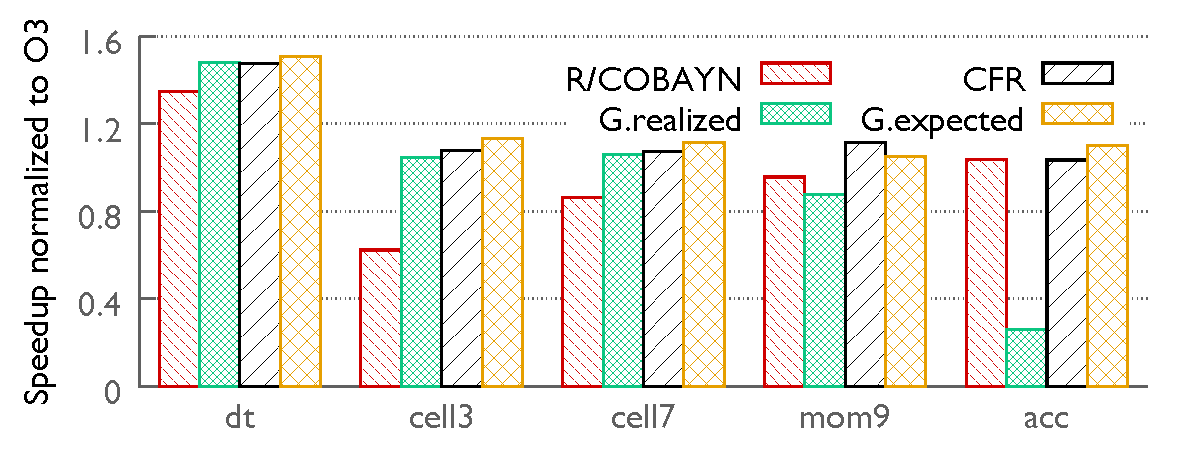
\includegraphics[width=0.6\textwidth]{gnuplot_temp/deep_dive.pdf}
\vspace{-6mm}
\caption{Normalized speedups for top-5 loops of Cloverleaf on Intel Broadwell.
Note: COBAYN (static) and R generated the same code in this case.}
\label{fig:case}
\vspace{-4mm}
\end{figure}


\vspace{.25em}
\noindent (2) Compiler phase ordering techniques \cite{Kulkarni:2012:MCO:2384616.2384628, Nobre:2016:GIC:2907950.2907959, Kulkarni:2004:FSE:996841.996863, 6662511, micomp}:
given a set of compiler optimization passes, there are many valid orders to apply each of them, which usually generate code variants with different runtime performance.
Our work focuses on the Intel tool chain, which does not provide command-line flags to perform phase ordering.
However, our approach may be applicable to Clang/LLVM, which supports such capability.
We plan to explore this in future work.


\begin{comment}
% search-based, random and genetic search
Random methods \cite{Chen:2010:EIO:1806596.1806647,opentuner} evaluate and select the best combination out of many randomly drawn in a uniform manner from the search space.
Chen et al. \cite{Chen:2010:EIO:1806596.1806647} conduct an in-depth study on a fundamental question of iterative compilation with random space search, i.e., program input sensitivity, with 1000 data sets for each benchmark.
They observe that a single optimization flag combination can achieve most of the best performance for a program across all the data sets for their benchmark suites.
So far, we do not consider input sensitivity as our primary objective, but we plan to look into it in the future.
Genetic algorithms \cite{Kulkarni:2004:FSE:996841.996863, 4625477} can also be used to search the flag combination space.
However, due to relatively high search overhead and resource limitations, we do not explore them in this work. Also, we consider our current approach to be more intuitive so that our results are easier to interpret that those derived from genetic algorithms that act as a black box.

% search-based, previous state-of-the-art
Pan et al. \cite{1611551} propose Combined Elimination (CE) to capture interactions among GCC compiler optimizations.
CE starts off with all compiler optimizations and eliminates those that introduce negative performance impacts in a greedy and iterative fashion.
It considers all 38 on/off flags of GCC 3.3.3 and treats a program as a whole.
Their experiments show CE effectively reduces the tuning overhead while achieving comparable performance results to prior approaches \cite{1191546, 1348305}.
In contrast, we take a fine-grained per-loop approach for both binary and multi-valued flags for latest Intel C/C++ Compiler tool chain.
Our evaluation also indicates CE performs worse than our approach.
\end{comment}

%and is not comparable to ours, either.
%Taken CE as the state-of-the art,
\begin{comment}
Cavazos et al. \cite{Cavazos:2007:RSG:1251974.1252540} show that CE is neither effective nor efficient for the EKOPath commercial compiler with 121 optimizations and is also worse than a random selection method, which is consistent with our experimental evaluations for ICC.
\end{comment}
% automated predictive modeling

\begin{comment}
Given a new program, CE tries to exploit the interactions among compiler optimizations implicitly with no reuse of prior knowledge, while machine learning techniques \cite{1611549, Cavazos:2007:RSG:1251974.1252540} build a model representing the prior knowledge to reuse for new applications.
Agakov et al. \cite{1611549} proposed two probabilistic models for a set of training programs.
The model can use an independent and identical distribution (IID) or a stationary Markov chain, which is learned by simply counting the occurrences of desired sub-sequences in the training optimization sequences.
Given a new program, their approach first extracts its static features and applies nearest-neighbor search to determine which learned probabilistic model is the best fit.
During the tuning stage, the desired number of samples can be drawn from the model.
Their experiments show that their approach can find good optimization sequences faster than a pure random search and genetic algorithm based search.
Cavazos et al. \cite{Cavazos:2007:RSG:1251974.1252540} collect hardware performance counters as feature sets to train a probabilistic model for optimization sequence selection.
Their work demonstrates the importance of using dynamic program features and a learned statistical model for prior knowledge in compiler optimization selection.
They also note that static features used in their previous work \cite{1611549} for small embedded kernel benchmarks are not effective for large applications with many dynamic branches.
We want to highlight that although predictive models \cite{1611549, Cavazos:2007:RSG:1251974.1252540} reduce tuning overhead, they do not improve the best achievable performance by random search while our approach does perform better and has the potential to improve these predictive models.
\end{comment}

\iffalse
% more automated predictive modeling
Modeling techniques have also employed logistic regression, neural network and multivariate adaptive regression splines \cite{Vaswani:2007:MSE:1251974.1252536, Cavazos:2007:RSG:1251974.1252540}, Bayesian networks \cite{6962349}, dependency trees \cite{Garciarena:2016:EOC:2908961.2931696}, probabilistic graphs \cite{Nobre:2016:GIC:2907950.2907959}, and stationary Markov chains \cite{1611549}.
These methods all try to implicitly capture the interactions and dependencies among compiler flags or compilation phases in order to focus search on the area with highest performance potential.
Program features can be estimated statically \cite{1611549} or dynamically with performance counters \cite{Cavazos:2007:RSG:1251974.1252540, 6962349, Leather:2009:AFG:1545006.1545059}.
%, and may be automatically extracted \cite{}.
Instead of utilizing program features to build models, our approach simply relies on per-loop time collected by light-weighted Caliper \cite{caliper} to implicitly capture the interactions of compiler flags on different compilation modules.
This relieves programmers from having to build complicated models before obtaining performance benefits for their target programs.
Moreover, a recent study \cite{FursinMGL15} utilizing crowd-sourcing compilation shows accuracy for machine-learning predictive models on large-scale datasets is close to that of a random guess.
Such a surprising result also raises a fundamental concern about machine-learning based approaches, namely, scarcity of training data, meaningful features, and validity of generalization, in addition to an inherent difficulty in interpreting learned models.
\fi

\iffalse
% manual predictive modeling
The interaction of compiler flags or phases can also be captured explicitly with expert knowledge.
Jantz et al. \cite{6662511} manually classified VPO optimization phases into cleanup phases, branch phases and non-branch phases.
After verifying the independence among branch phases and non-branch phases, they divide the phases into two disjoint groups and show extreme effectiveness of utilizing phase interaction information to reduce the search space size by 96.75\% while achieving almost the same performance as previous search-based techniques.
However, such an expert characterization process is very time consuming and may not be feasible for production quality compilers like ICC, GCC and LLVM, while our method is readily applicable.
\fi

\begin{comment}
% Domain-specific and architecture-specific tuning
The aforementioned compiler-based tuning techniques are general in the sense they do not take advantage of domain knowledge of programs being tuned.
Zhang et al. \cite{frank2012, frank2013} propose an auto-tuner for 3D stencil code generation on several heterogeneous GPUs.
They exhaustively search a space composed of GPU thread block dimensions and memory placement.
In \cite{5161004, Tiwari:2009:SAF:1586640.1587552}, Tiwari et al. propose a domain-specific language (DSL) for compilation transformation recipes.
Their framework tunes each computation kernel separately and requires experts to write valid recipes in their DSL while our framework tunes multiple kernels simultaneously via compiler command-line flags, a process that can be fully automated.
\end{comment}

\iffalse
% others
Sourouri et al. \cite{sc2017} employ dynamic voltage and frequency scaling (DVFS) on Intel Xeon multi-core machines to tune each kernel of their seismic wave propagation application.
They exhaustively search a space composed of core and uncore frequency, number of OpenMP threads and then enforce the best per-kernel configuration via runtime library for energy-saving.
Others have also investigated runtime adaption techniques to account for performance discrepancies incurred by power caps \cite{cluster2016} or to impose different tuning objectives.
%that can be indiuser's disposal.
Our approach focuses on compile-time flag composition and is orthogonal to their work.
\fi

\section{Conclusion} \label{conclusion}

% approach and effectiveness
In this work, we presented a fine-grained per-loop compiler flag
selection framework, \toolname, that combines program profiling and
search space focusing algorithms to improve performance of parallelized
scientific programs, in which different code regions/loops may be optimized
with different flags.  Our experimental evaluation shows that
\toolname's Caliper-guided Random Search (CFR) effectively utilizes
collected per-loop runtimes to focus the search on performant program
compilation configurations.
%and is able to tolerate measurement errors.
\toolname achieves a 9.2\% to 10.3\% (geometric mean) performance improvement
in comparison to O3 baseline, outperforms state-of-the-art random search
algorithms by 4.6\% to 5.6\%, and is better than machine-learning based approaches by 4.6\%.
%which also has the potential to improve future predictive modeling techniques.
We also showed that greedily picking the per-loop best compilation vectors often
degrades program performance due to complex inter-module dependencies, and
fine-grained random search without guidance of runtime information does not
guarantee performance improvements.
% insight and take-away


\if 0
\section{First Section}
\subsection{A Subsection Sample}
Please note that the first paragraph of a section or subsection is
not indented. The first paragraph that follows a table, figure,
equation etc. does not need an indent, either.

Subsequent paragraphs, however, are indented.

\subsubsection{Sample Heading (Third Level)} Only two levels of
headings should be numbered. Lower level headings remain unnumbered;
they are formatted as run-in headings.

\paragraph{Sample Heading (Fourth Level)}
The contribution should contain no more than four levels of
headings. Table~\ref{tab1} gives a summary of all heading levels.

\begin{table}
\caption{Table captions should be placed above the
tables.}\label{tab1}
\begin{tabular}{|l|l|l|}
\hline
Heading level &  Example & Font size and style\\
\hline
Title (centered) &  {\Large\bfseries Lecture Notes} & 14 point, bold\\
1st-level heading &  {\large\bfseries 1 Introduction} & 12 point, bold\\
2nd-level heading & {\bfseries 2.1 Printing Area} & 10 point, bold\\
3rd-level heading & {\bfseries Run-in Heading in Bold.} Text follows & 10 point, bold\\
4th-level heading & {\itshape Lowest Level Heading.} Text follows & 10 point, italic\\
\hline
\end{tabular}
\end{table}


\noindent Displayed equations are centered and set on a separate
line.
\begin{equation}
x + y = z
\end{equation}
Please try to avoid rasterized images for line-art diagrams and
schemas. Whenever possible, use vector graphics instead (see
Fig.~\ref{fig1}).

\begin{figure}
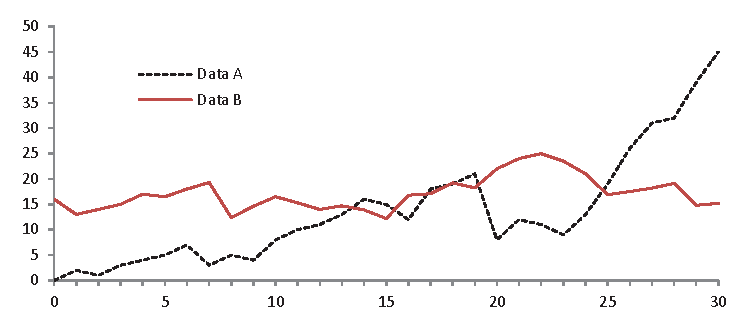
\includegraphics[width=\textwidth]{fig1.eps}
\caption{A figure caption is always placed below the illustration.
Please note that short captions are centered, while long ones are
justified by the macro package automatically.} \label{fig1}
\end{figure}
\fi

\if 0
\begin{theorem}
This is a sample theorem. The run-in heading is set in bold, while
the following text appears in italics. Definitions, lemmas,
propositions, and corollaries are styled the same way.
\end{theorem}
%
% the environments 'definition', 'lemma', 'proposition', 'corollary',
% 'remark', and 'example' are defined in the LLNCS documentclass as well.
%
\begin{proof}
Proofs, examples, and remarks have the initial word in italics,
while the following text appears in normal font.
\end{proof}

For citations of references, we prefer the use of square brackets
and consecutive numbers. Citations using labels or the author/year
convention are also acceptable. The following bibliography provides
a sample reference list with entries for journal
articles~\cite{ref_article1}, an LNCS chapter~\cite{ref_lncs1}, a
book~\cite{ref_book1}, proceedings without editors~\cite{ref_proc1},
and a homepage~\cite{ref_url1}. Multiple citations are grouped
\cite{ref_article1,ref_lncs1,ref_book1},
\cite{ref_article1,ref_book1,ref_proc1,ref_url1}.
\fi
%
% ---- Bibliography ----
%
% BibTeX users should specify bibliography style 'splncs04'.
% References will then be sorted and formatted in the correct style.

%\bibliographystyle{splncs04}
\bibliographystyle{splncsnat}
\bibliography{ref.bib}

\if 0
\begin{thebibliography}{8}

\bibitem{ref_article1}
Author, F.: Article title. Journal \textbf{2}(5), 99--110 (2016)

\bibitem{ref_lncs1}
Author, F., Author, S.: Title of a proceedings paper. In: Editor,
F., Editor, S. (eds.) CONFERENCE 2016, LNCS, vol. 9999, pp. 1--13.
Springer, Heidelberg (2016). \doi{10.10007/1234567890}

\bibitem{ref_book1}
Author, F., Author, S., Author, T.: Book title. 2nd edn. Publisher,
Location (1999)

\bibitem{ref_proc1}
Author, A.-B.: Contribution title. In: 9th International Proceedings
on Proceedings, pp. 1--2. Publisher, Location (2010)

\bibitem{ref_url1}
LNCS Homepage, \url{http://www.springer.com/lncs}. Last accessed 4
Oct 2017
\end{thebibliography}
\fi
\end{document}
